
\documentclass[conference]{IEEEtran}

\usepackage{float} 
\usepackage{url}  
\usepackage{multirow}
\usepackage{caption}
\usepackage{subcaption}
\usepackage{booktabs}
\usepackage{cite}
\pagestyle{plain}
\usepackage{amsmath}
\usepackage{float}
\usepackage{tikz}
\usetikzlibrary{shapes.geometric, arrows, positioning}
\usepackage{placeins}
\usepackage{comment}

\ifCLASSINFOpdf
  \usepackage[pdftex]{graphicx}
\fi

\hyphenation{op-tical net-works semi-conduc-tor}

\begin{document}


\title{Lacuna Solar Survey Challenge: Counting Photovoltaic and Solar Panels from Aerial Imagery}

\author{\IEEEauthorblockN{\\ Hugo Veríssimo}
\IEEEauthorblockA{Complements of Machine Learning 24/25\\
University of Aveiro\\
Aveiro, Portugal\\
hugoverissimo@ua.pt}
\and
\IEEEauthorblockN{\\ João Cardoso}
\IEEEauthorblockA{Complements of Machine Learning 24/25\\
University of Aveiro\\
Aveiro, Portugal\\
joaopcardoso@ua.pt}}

\maketitle
\thispagestyle{plain}

\begin{abstract}
abstact
\end{abstract}

\begin{quote}
\small
\noindent
\textbf{Keywords:} R, Object Detection
\end{quote}

\IEEEpeerreviewmaketitle


\section{Introduction}

Access to electricity and warm water has been a basic necessity for a long time in the developed world. In developing countries, the lack of a centralized distribution system makes this access harder for everyone. To improve on this gap, it is essential for governments, non-governmental organizations, and energy suppliers to understand how solar photovoltaic and solar thermal panels (for electricity and water heating, respectively) are distributed throughout the territory to ensure proper planning and effective policy making. In this context, a challenge was created by the Lacuna Fund and associate entities in the Zindi platform to develop a machine learning model capable of accurately detecting and counting the number of solar thermal (solar from here on) and photovoltaic panels in drone and satellite imagery.

In the present work, we have developed different approaches to the problem at hand, where we need to count the two types of panels separately: taking a regression type approach, where images are analysed as a whole and the target number of panels are provided per image; by identifying the panels through object detection and counting them afterwards; and by applying segmentation models to identify the regions of interest, analysing them and counting the panels. The different approaches were developed so that a single model for each type would be able to tackle the task of identifying and counting the different panels.

%EXPLICAR E FICAR BEM EXPLICITO: DUAS REGRESSOES: pan E boil

\section{State of The Art}

The task of detection of solar panels serves many purposes, with the strongest focus of the works here documented being on the detection and localization of solar panels in large areas (countries). This type of assessment allows for proper planning of infrastructure, and to adapt current maintenance through peak output of dense areas with solar panels.

In the work of Malof \textit{et al.} the authors developed an automatic detection model of solar arrays, specific for photovoltaic panels. The model developed had computational efficiency at the forefront, with the purpose of being deployed nation wide in the United States, hence a multi-stage approach consisting of: pixel-wise feature extraction; Random Forest (RF) Classifier; post-processing to improve the pixel-wise classification accuracy for the object detection phase; finalizing with the object detection, via thresholding the finalized confidence map. This algorithm presents superior performance to standalone RF, and was well remarked as an initial assessment methodology for large areas. 

The \textit{DeepSolar} model consists allowed to create a nearly complete contiguous solar panel installation map, and consists of two parts, with different purposes: firstly, via transfer learning the convolutional neural network (CNN) classifier is trained on labeled imagery that merely indicates the presence or absence of panels (though the volume of data is considerable, at almost 400 000 images just for this task). The model is then enhanced by adding an additional CNN branch directly connected to the intermediate layers to add segmentation capabilities to the model. The difference is that this approach allows the model to be trained on the same dataset, to "greedily" extract the relevant features associated with solar panels, learning in a semi-supervised manner. The model was able to achieved the best result of 93.7 \% precision and 90.5 \% recall in non-residential areas.

Different models have been proposed for panel detection through image segmentation, using Mask R-CNN {He, 2020}, TernausNet, based on U-Net {Kausika 2021}, MobileNet with U-Net backbone {Wari, 2021}, with different approaches to data preparation and application. These models consistently score higher than 90 \% in terms of precision, at the cost of higher computation times compared to the examples previously mentioned (also for very different task sizes). A couple notable aspects across publications: the size of datasets (often in the tens of thousands of images), with strong strategies for collecting and/or preprocessing, ensuring that the models have the best possible starting point to learn and develop; and the focus on a specific type of panel or problem topic, not trying to solve multiple problems with a single tool.

For the purpose of this work, we have developed three approaches to the problem, to assess their strengths and merits, which will be detailed in the next subsections.

\subsection{Image-based Regression}

Considering that every image is labelled in terms of amount of photovoltaic and thermal solar panels, the conditions for training considering a regression approach are available. For this, deep neural networks (convolutional neural networks, CNN) were considered for their excellent capabilities in extracting spatial features, but each with a distinguishing feature.

ResNet (Residual Networks) was introduced in 2015 by Microsoft, and is notorious for dealing with vanishing gradient problem by skipping connections between neuron layers. This allows the model to grow and have several layers (over 100), making it capable of learning a larger variety of features from the first to the deeper layers, without suffering from performance degradation.

DenseNet follows on the footsteps of ResNet, and was introduced in 2016 by Huang \textit{et al.}, whereby the idea of skipping connections is taken further, and every layer prior to a given layer is connected to it. This avoids the chain multiplication problem (which leads to vanishing gradients), while reusing previously learned features, retaining relevant information throughout the deepness of the CNN. This architecture also has the benefit of using less parameters than CNN in general (and ResNet as well).

EfficientNet (EffNet), the most recent of this group was introduced by Google AI in 2019, and departs from the direct implementation of the aforementioned methods, dealing with vanishing gradients given its intrinsic architecture. By having MB Conv (Mobile Inverted Bottleneck Convolution) as its building block, it allows to extract spatial features by expanding the number of channels to perform depthwise convolution and applying separate filters per channels \textbf{(verificar a nomenclatura)}, that is then compressed to the original size of the input. Whilst this happens, the mechanism of squeeze-and-excitation determines the importance of said features, further addressing the vanishing gradient problem. This architecture is then scaled via compound scaling (rather than arbitrarily), whereby the size of the CNN (depth x width and input resolution) is scaled in a balanced manner, with the compound coefficient $\phi$ being adjusted by grid search.

\subsection{Object Detection}

With object detection, the model is trained based on bounding boxes surrounding the subject of interest, in order to be able to identify them in new environments and types of images. With multiple classes, the model discern between labels with class probabilities, estimated from the extracted features of the assessed boxes (using a CNN) throughout the image. One of the most famous and used models is YOLO ("You Only Look Once") introduced in 2015 by Redmon \& Fardhi, being a crucial model in fast object detection and localization. In a single stage, the model addresses the localization and detection problems, where a CNN backbone (that has changed with the released versions) is used, with feature fusion layers (akin to the way learned features are reused, involving various algorithms), and an output of the likelihood of a class and the location of the bounding boxes.

\subsection{Instance Segmentation}

Building on the concepts presented before on object detection, instance segmentation addresses the problem of identification by incorporating the information of object masks. These are tighter around the object (than bounding boxes), which serve to add a layer to the YOLO algorithm. A global prototype mask (that works with a separate, smaller CNN) is generated for the whole image - this way once the bounding box is determined, mask coefficients are estimated in order to combine the prototype masks into an instance specific mask. This approach avoids per mask full resolution segmentation, keeping the model size small and fast.



\section{Methodology}

\subsection{Dataset \& EDA}

The dataset was provided within the Zindi challenge, consisting of 4419 images (from drone and satellite sources), and per image metadata, consisting of the source (drone or satellite), mask placement, and context of the installation surroundings (e.g., roof, floor, array).\textbf{info do pie chart} The proportion between photovoltaic and thermal solar panels is heavily imbalanced, with 95 \% of the dataset corresponding to photovoltaic panels.
%o dados, fornecidos pela propria competicao (citar), consistem em 4419 imagens, complementadas por metadata referente à origin da imagem e ao placement dos paineis, providing context on installation environments.
Of all the images, 3312 (75 \%) have detailed information on the masks (location, number of panels within, if they are photovoltaic or thermal). The remaining 1107 (25 \%) do not have this information, only the number of photovoltaic and thermal panels in the image. Hence, per design of the competition the train/test split is 75/25.

%da totalidade destas imagens, 3312 (75\%) contêm indicacoes das delimitacoes de conjutnos de paineis e de boilers, atraves de poligonos, assim como a quantidade que se encontra dentro de cada qual. as restantes 1107 (25\%) nao têm esta informacao. Assim, por opcao da competicao, temos uma distribuicao de treino e teste de 75/25

\begin{figure}[H]
    \centering
    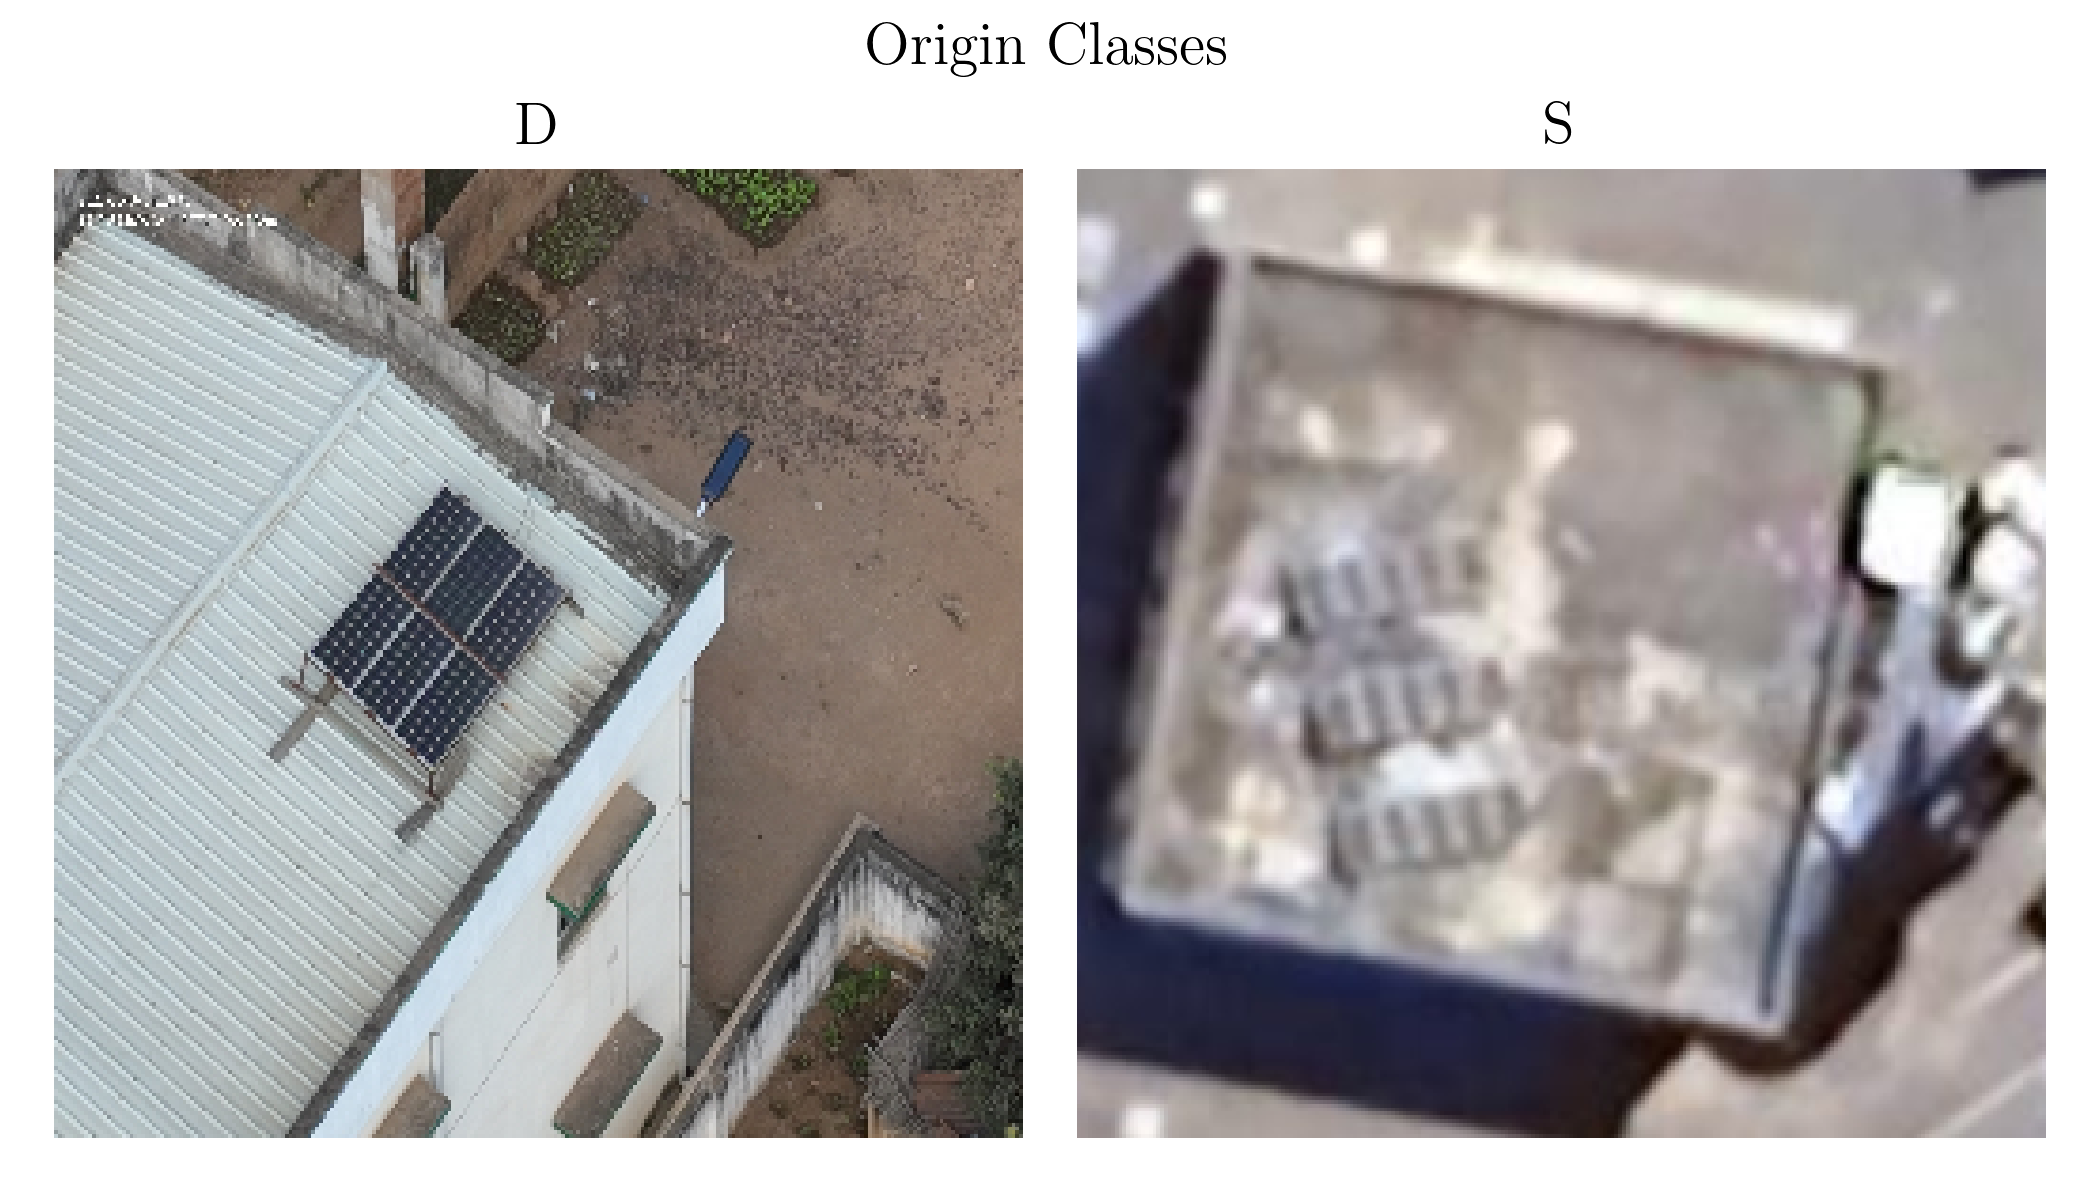
\includegraphics[width=1\linewidth]{assets/data_origin_classes.png}
    \caption{Images of photovoltaic panels placed on the roof, from drone (left side) and satellite (right side). The difference in resolution between them is evident.}
    \label{fig:data_origin_classes}
\end{figure}

\begin{figure}[H]
    \centering
    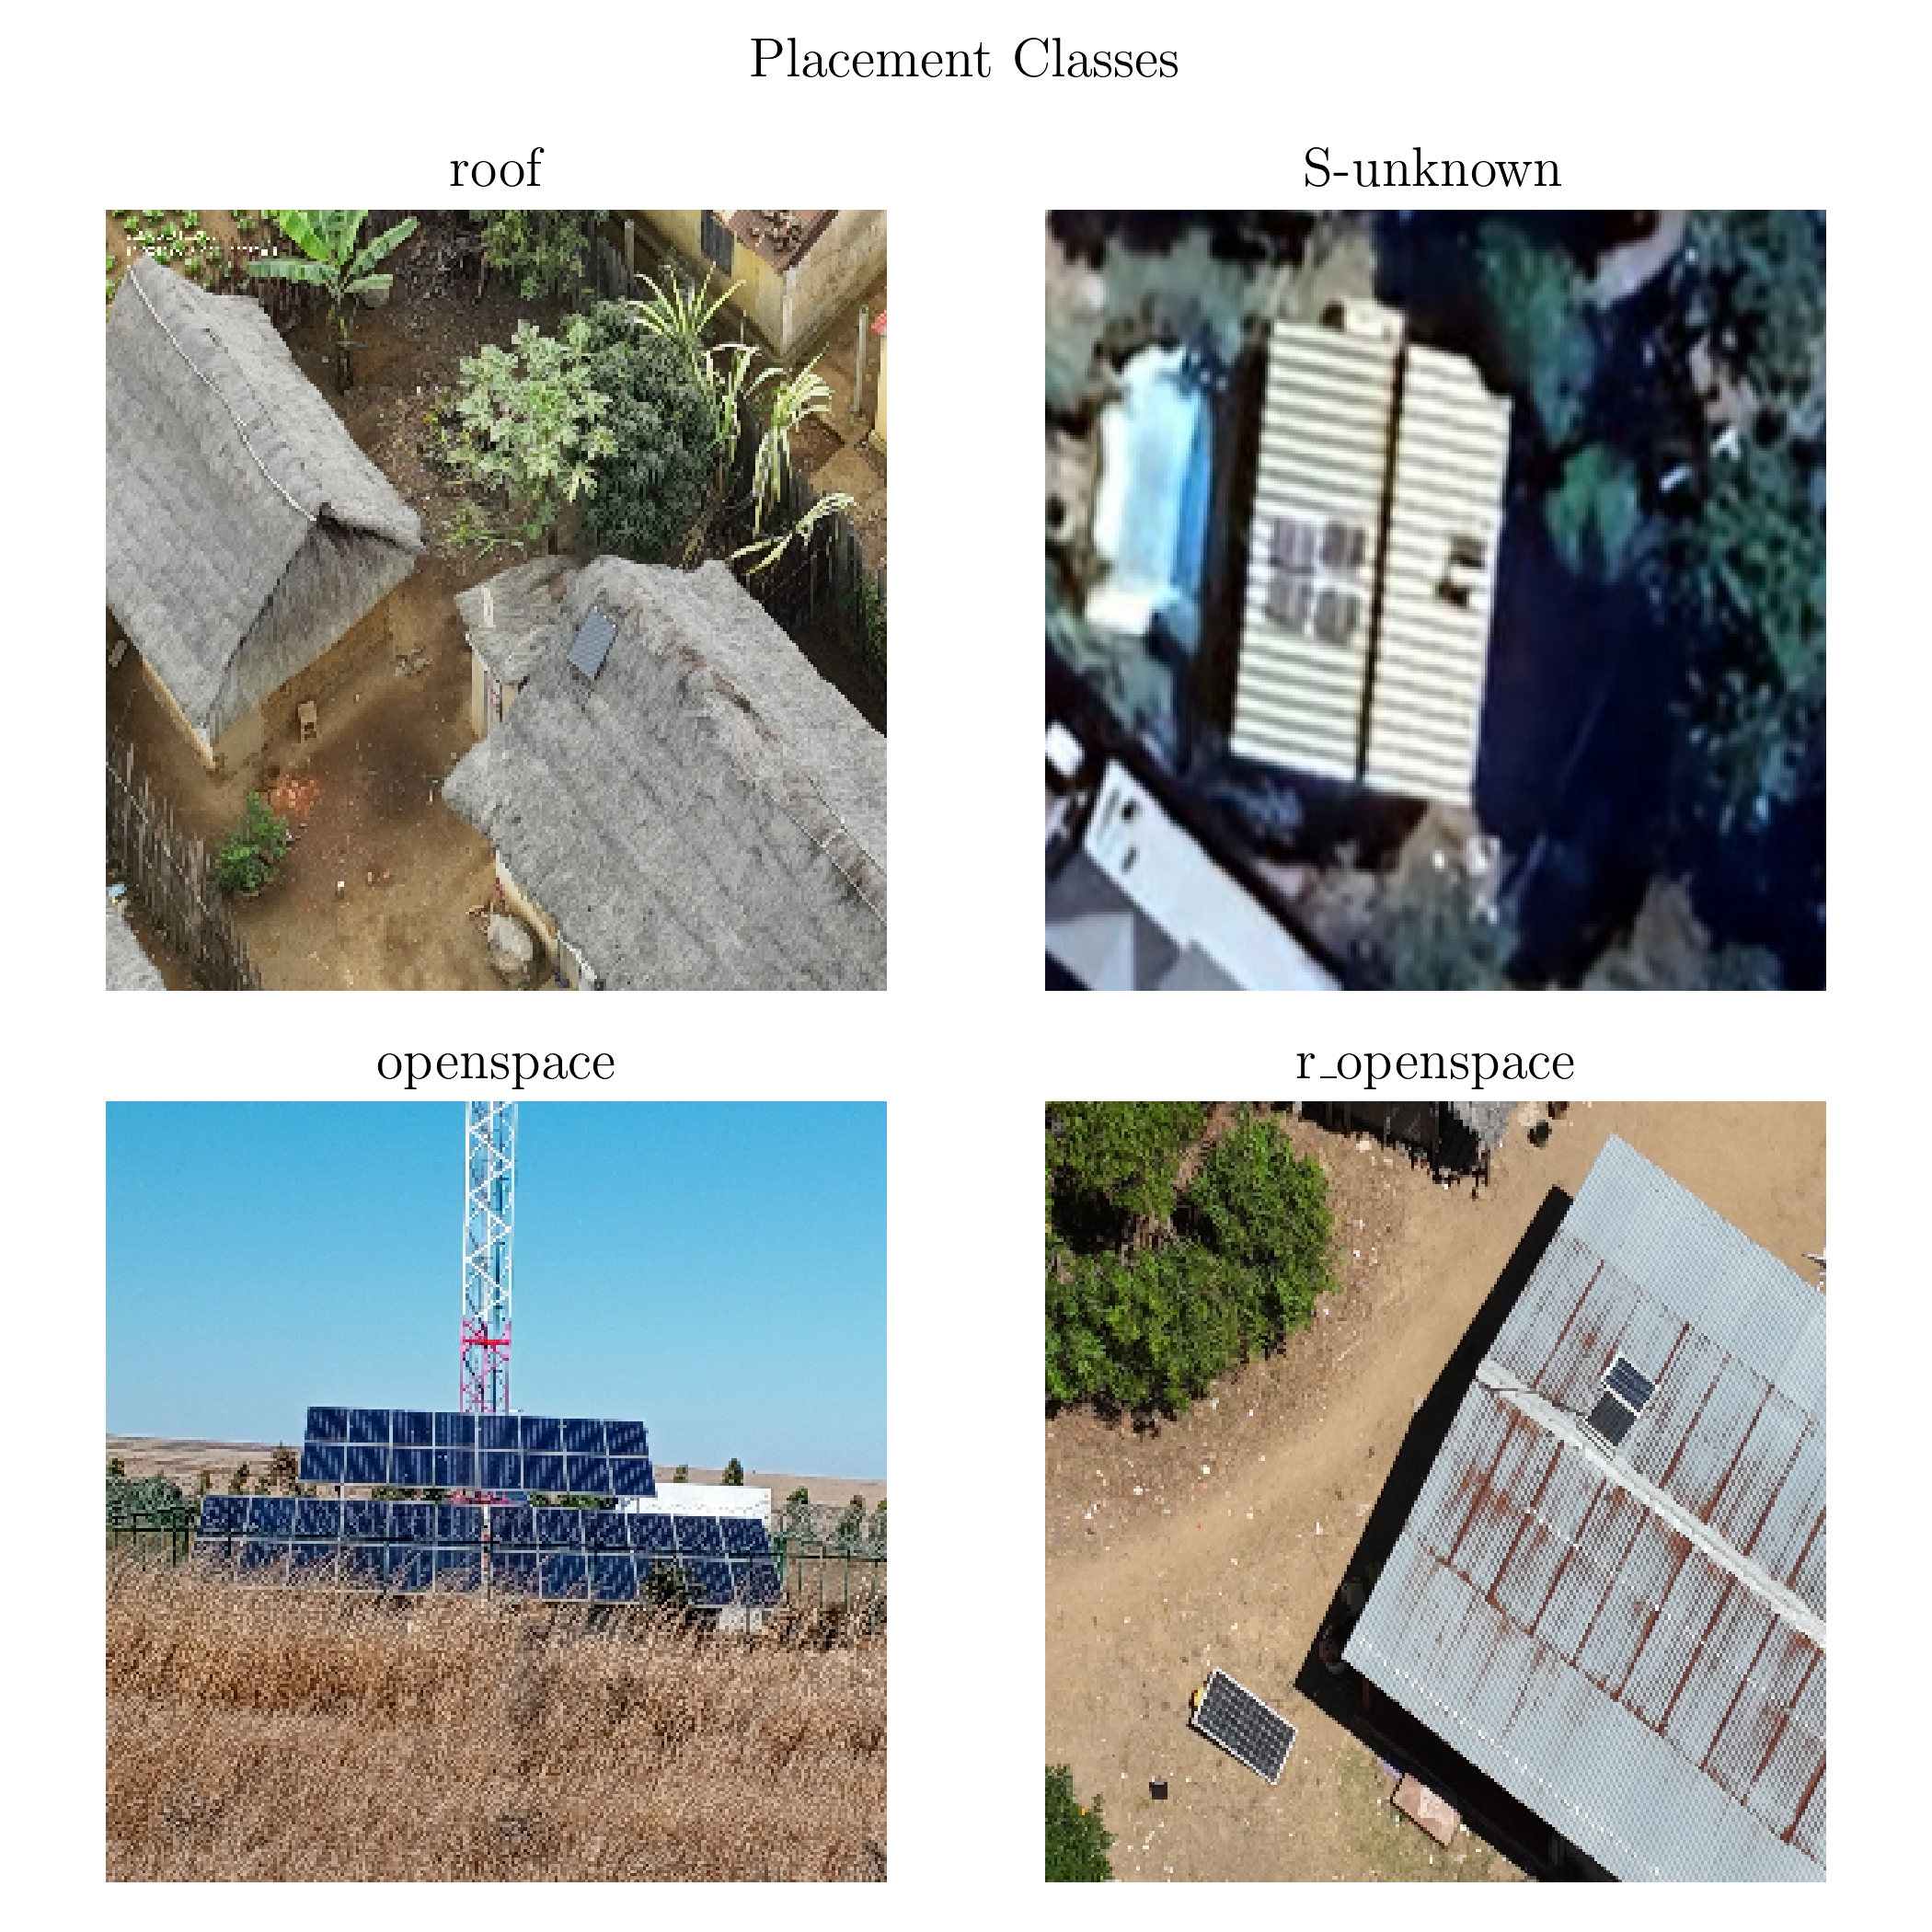
\includegraphics[width=1\linewidth]{assets/data_placement_classes.png}
    \caption{The different panel placement possibilities (top right is from satellite imagery). Bottom left image shows an image that is atypical for a drone style image.}
    \label{fig:data_placement_classes}
\end{figure}

In Fig. \ref{fig:data_placement_classes} the image origin and placement are displayed, which according to the challenge information were labelled by expert personnel. Where the placement class wasn't conclusive, the images are labelled as "S-unknown" (the remaining examples are self explanatory). Besides the two classes to be identified, the context and origin of the images means a considerable number of combinations for the model to learn, where some of these combinations might (and certainly are), under-represented given the relatively small dataset.

%nas figuras \ref{fig:data_origin_classes} e \ref{fig:data_placement_classes} podem-se observar as classes de origin e de placement relativas as imagens. as origins da imagem podem ser drone image (D) or satellite image (S), while the placement classes (Installations) sao distribuidas por on rooftops or terraces (roof), satellite images where the specific placement could not be determined (S-unknown), in open courtyards or gardens (openspace), that span both rooftops and outdoor spaces (r\_openspace).

\begin{figure}[H]
    \centering
    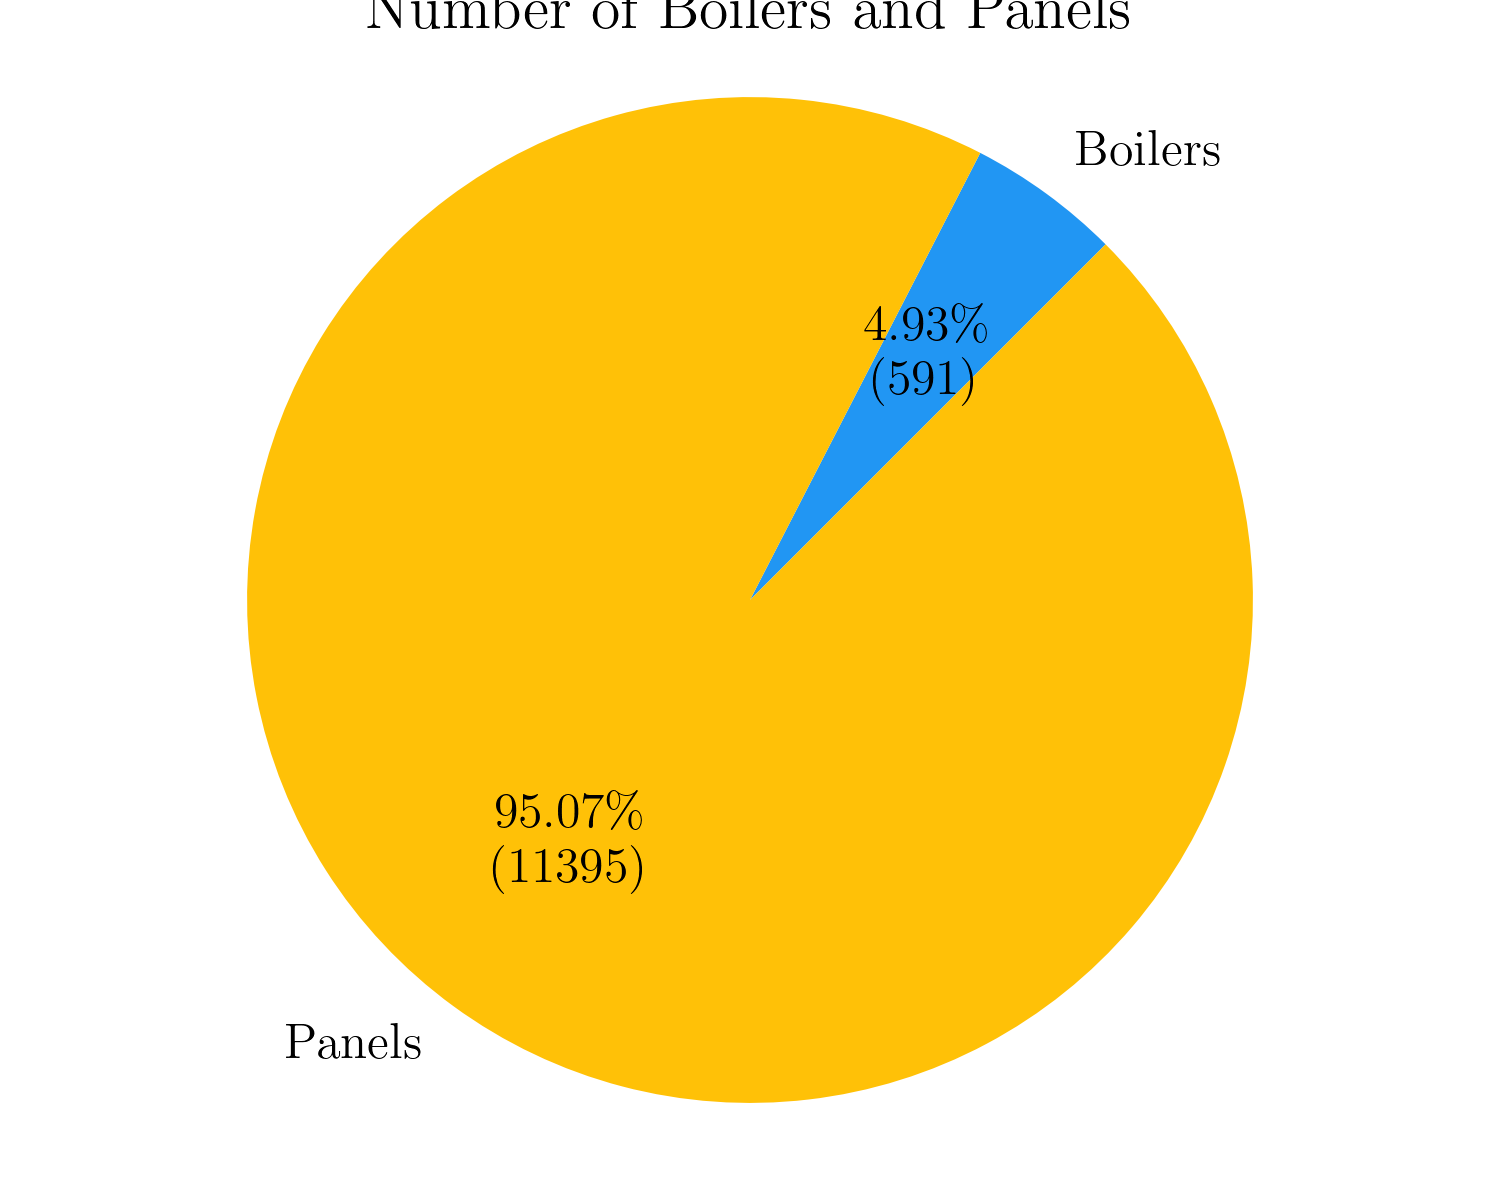
\includegraphics[width=1\linewidth]{assets/data_distribution.png}
    \caption{Portion of the number of photovoltaic and thermal solar panels counted from the available metadata.}
    \label{fig:data_distribution}
\end{figure}

%ademais, é também importante referir uma presença em maior peso de panels face ao numero de boilers, como se verifica na figura \ref{fig:data_distribution}

The masks are not consistent throughout the dataset, with varying number of panels within them (some contain a single panel, others might contain a complete array of up to 200), which can be clearly seen in Fig. \ref{fig:data_objectdistribution}.

\begin{figure}[H]
    \centering
    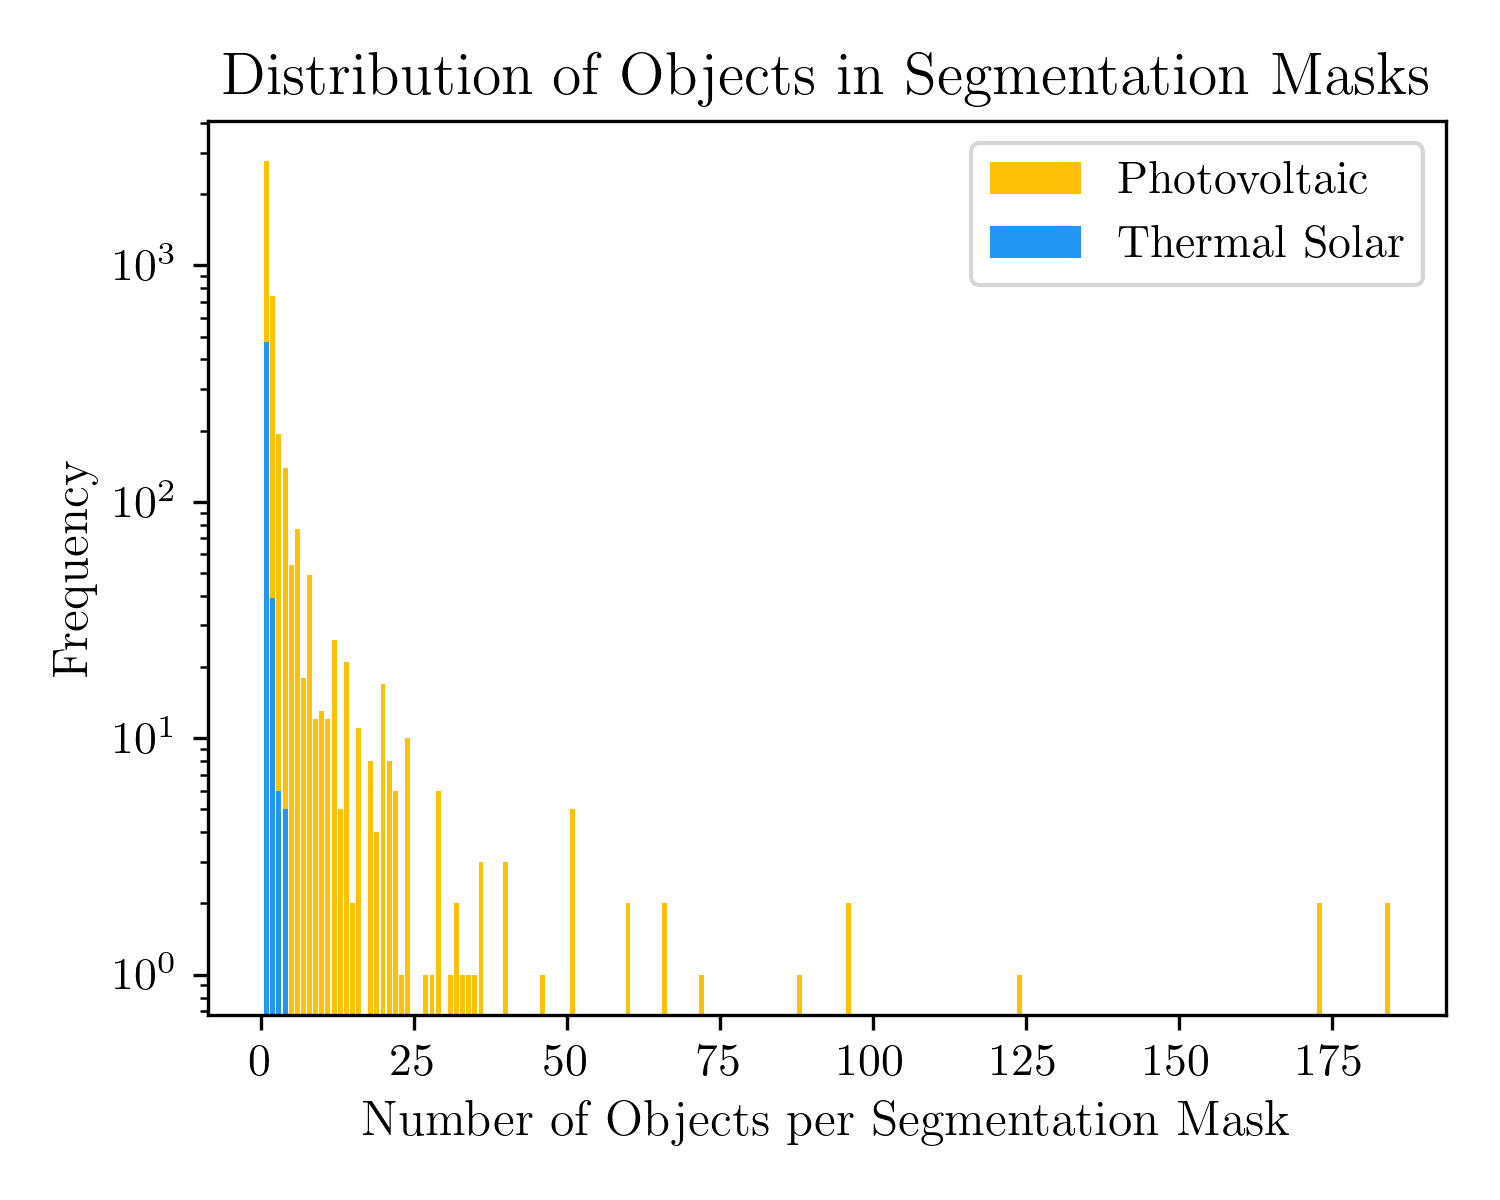
\includegraphics[width=1\linewidth]{assets/data_objectdistribution.png}
    \caption{Distribution of the number of panels within a single mask.}
    \label{fig:data_objectdistribution}
\end{figure}

%\begin{figure}[H]
%    \centering
%    \begin{subfigure}[b]{\linewidth}
%        \centering
%        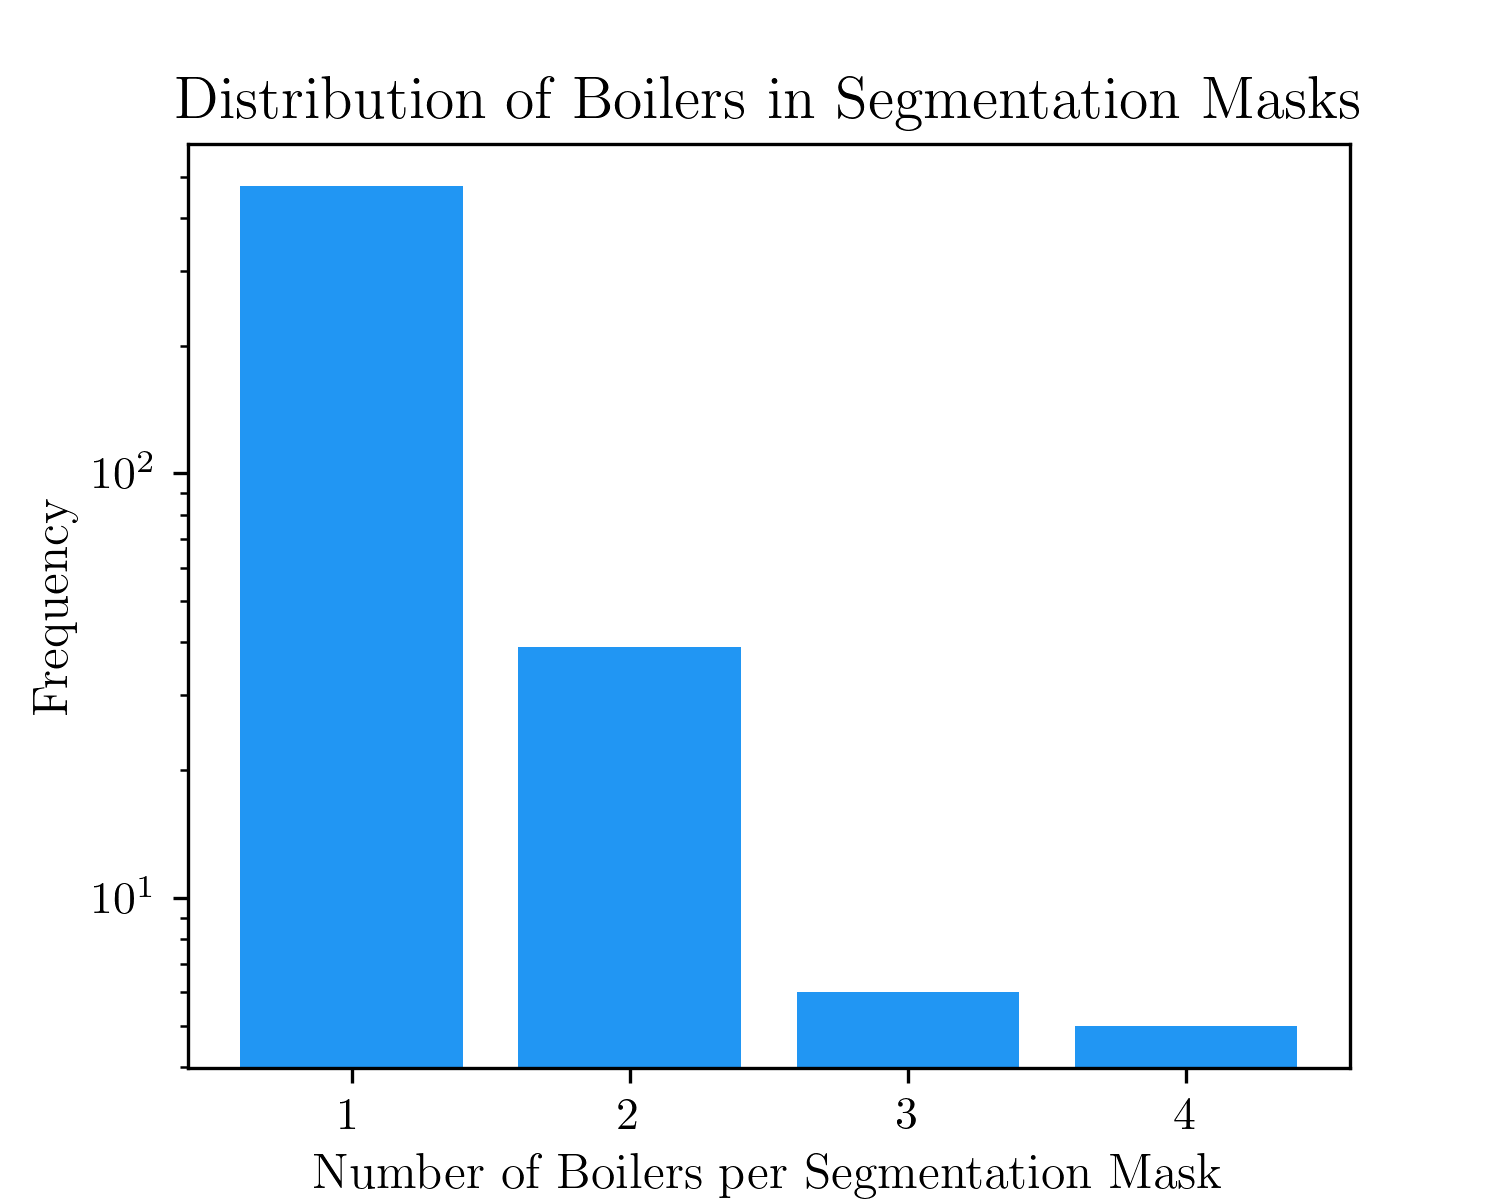
\includegraphics[width=\linewidth]{assets/data_boil_distribution.png}
%        \caption{Distribution of the number of thermal solar panels per segmentation mask.}
%        \label{fig:data_boil_distribution}
%    \end{subfigure}
%
%    \vspace{0.5em} % Optional spacing between images
%
%    \begin{subfigure}[b]{\linewidth}
%        \centering
%        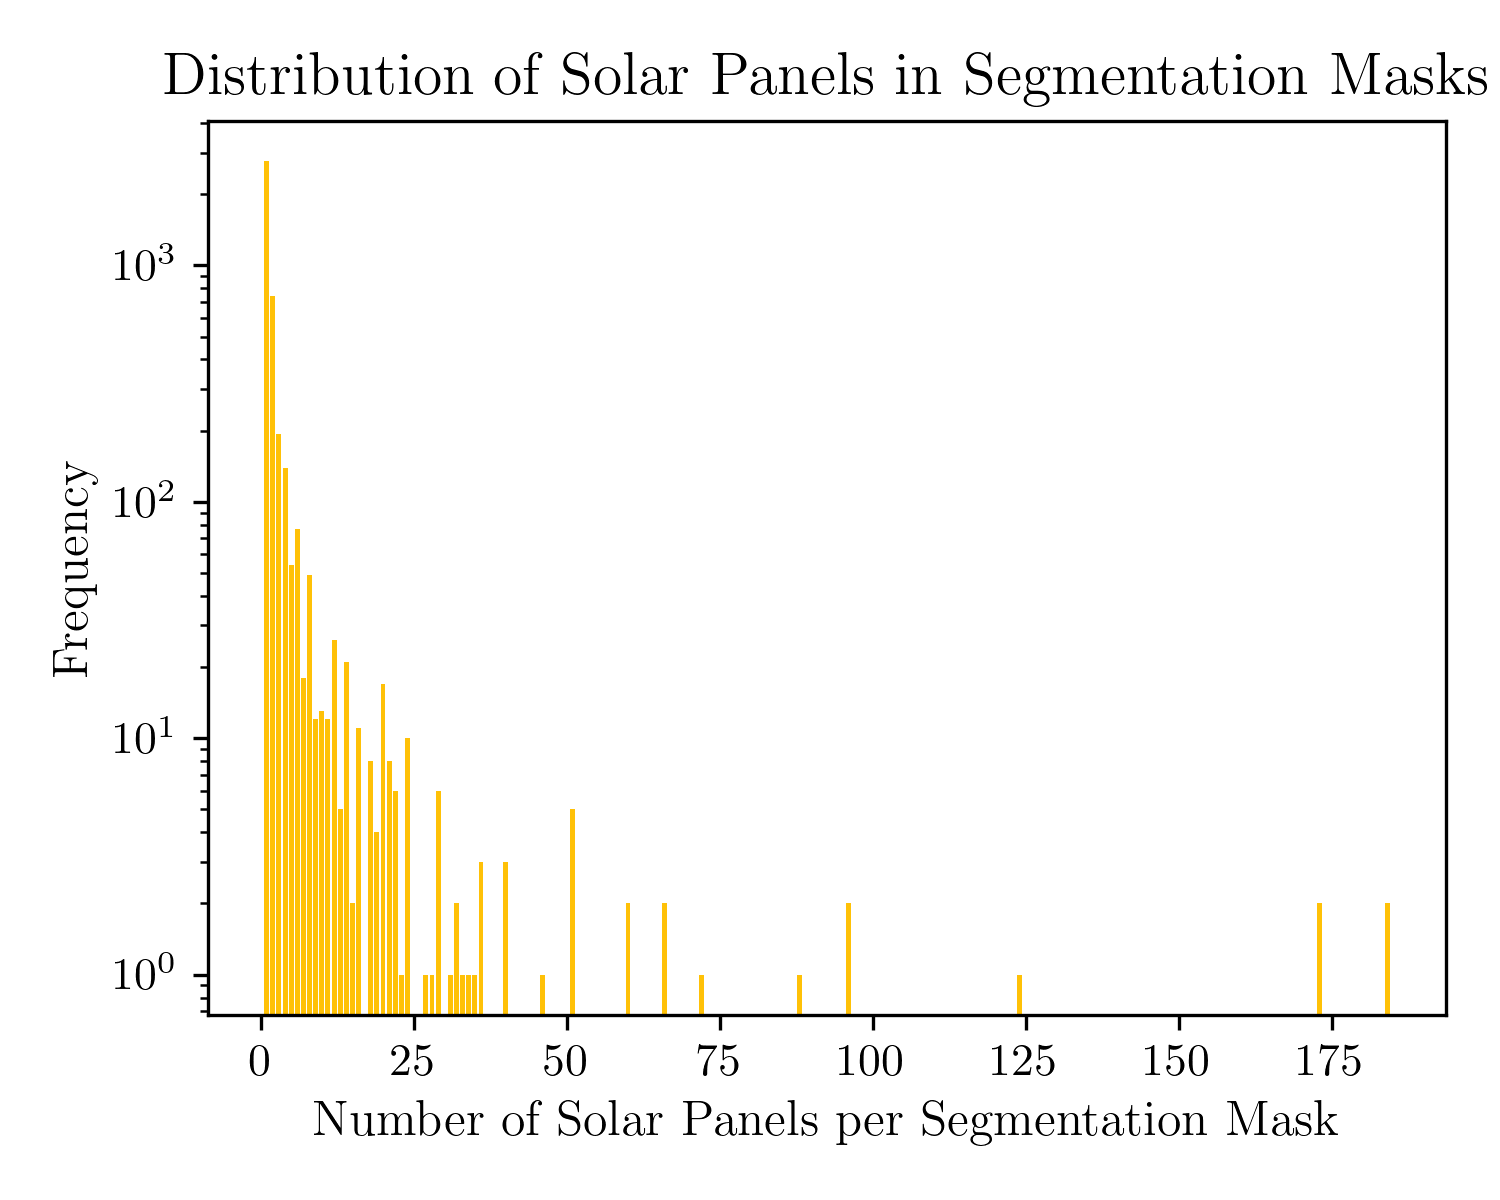
\includegraphics[width=\linewidth]{assets/data_panel_distribution.png}
%        \caption{Distribution of the number of photovoltaic panels per segmentation mask.}
%        \label{fig:data_panel_distribution}
%    \end{subfigure}
%    \caption{Distribution of the number of panels within a single mask.}
%    \label{fig:combined_data_distributions}
%\end{figure}

From the sample images below, the difference in the quality of the masks is stark. Several images were found to have misaligned vertices of the masks, and several masks had a large amount of panels (as seen from the distribution aforementioned). In principle, with the reference of the number of panels within each mask, it might have a small impact for some types of models, but the same model is in fact learning features for different representations: rather than for the representation of individual panels. This was an evident obstacle to the implementation of YOLO type models, which was dealt with, and further detailed below.

\begin{figure}[H]
    \centering
    \begin{subfigure}[b]{\linewidth}
        \centering
        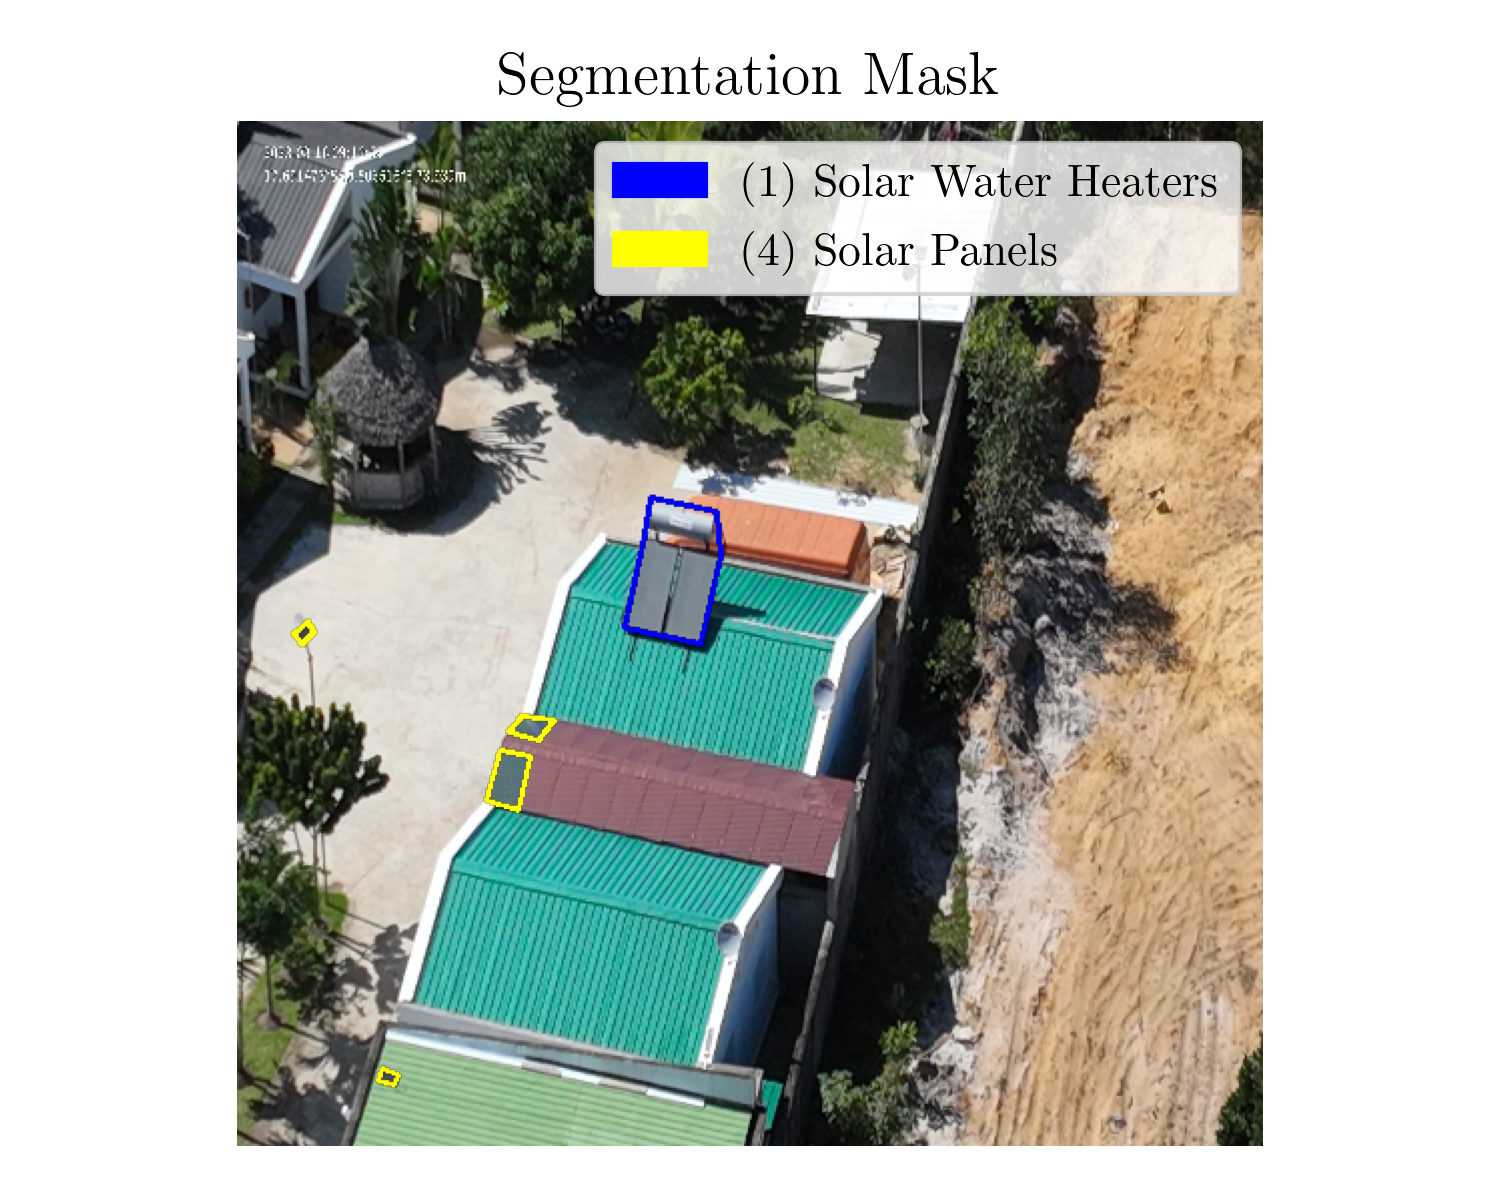
\includegraphics[width=\linewidth]{assets/data_segmentation_mask.png}
        \caption{Sample image of accurate labelling, with a single panel per mask.}
        \label{fig:data_segmentation_mask}
    \end{subfigure}

    \vspace{0.5em}

    \begin{subfigure}[b]{\linewidth}
        \centering
        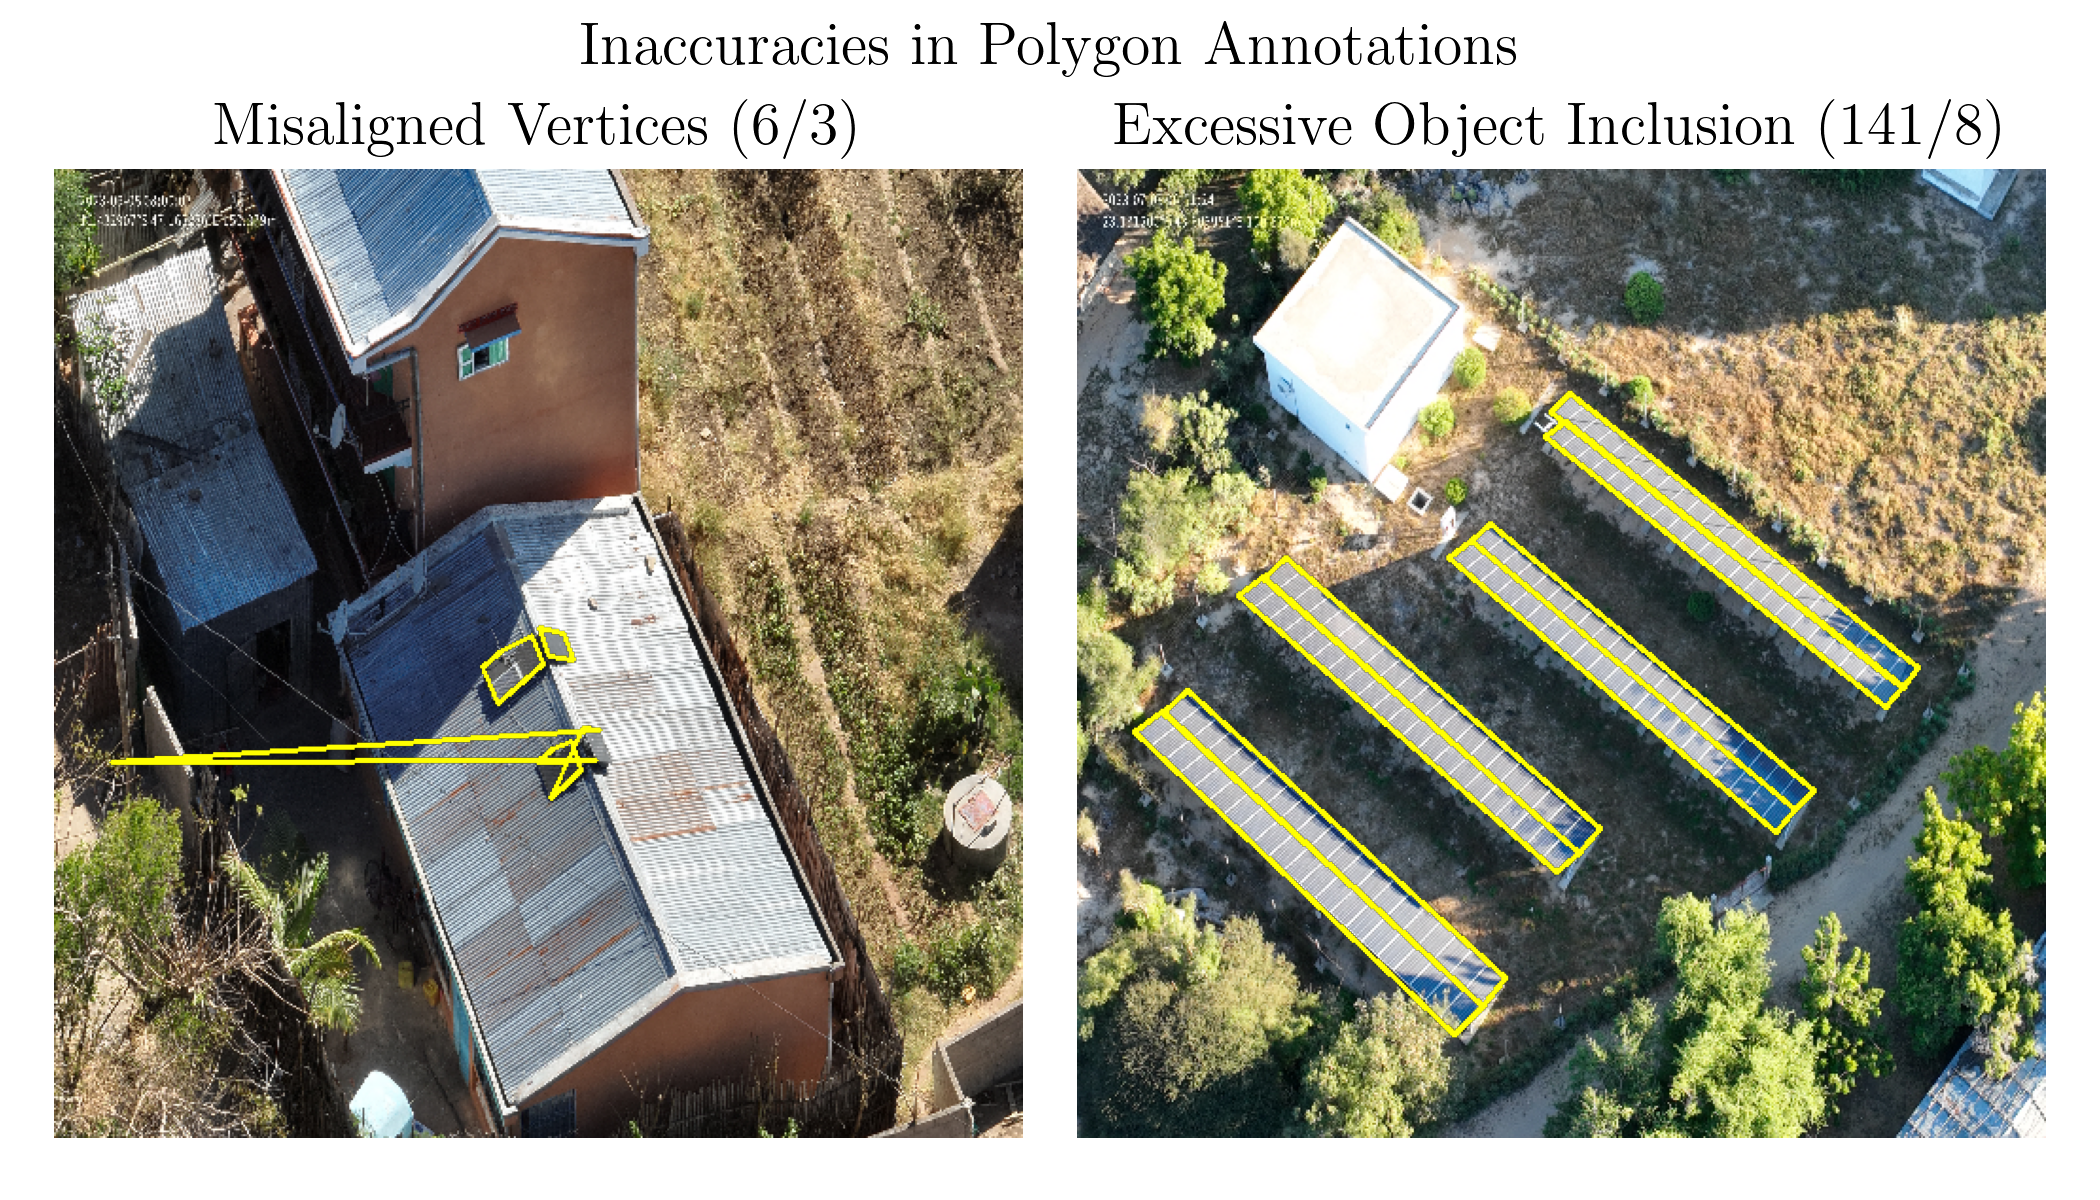
\includegraphics[width=\linewidth]{assets/data_poly_problems.png}
        \caption{Sample images of incorrectly marked masks: (on the left) mask distorted, misrepresenting the panel; (on the right) excessive objects within a single mask.}
        \label{fig:data_poly_problems}
    \end{subfigure}
    \caption{Sample images from the Zindi dataset.}
    \label{fig:combined_segmentation_poly_issues}
\end{figure}


%por fim, na imagem \ref{fig:data_segmentation_mask} pode-se verificar uma das imagens de treino e os respetivos poligonos referentes aos paineis e boilers convertidos numa mascara de segmentacao, onde se verifica a presença de 4 grupos de solar panels, sendo cada um destes um grupo unitário, e 1 grupo de boilers, tambem unitario.


\subsection{Preprocessing}

The discussion forum for the competition was a fruitful source of information on the dataset and how to address it. As seen above, the incorrectly defined masks, and the masks with several panels represented hindrances to achieve the best possible performance. Besides that, some of the masks were shifted from the actual position of the panels, which considering that all were identically shifted, seemed deliberate from the competition. By manually analysing every image  it was possible to detect such images (with wrongly drawn masks and shifted), and correct them. Upon completing the dataset revision, 263 of the training samples were lost due to poorly drawn masks (the remaining images that had misaligned masks were corrected).

%atraves de algumas discussoes do forum da competicao, uma analise mais aprofundada de algumas imagens aleator e dos dados de treino, foram verficados alguns obstaculos para a aplicacao dos modelos.

%nomeadamente, haviam linhas por poligono ao inves de linhas por imagem, as coordenadas dos poligonos eram strings ao inves de floats e algumas coordenadas tinham letras pelo meio.


%apos estas correções, uma das dificuldades tornou-se a validade dos poligonos. alguns poligonos tinham deslocacoes em relacao a posicao real dos paineis, outros tinham vertices misaligned, como se pode ver na imagem \ref{fig:data_poly_problems} alguns exemplos. apesar de não ser um erro o excessive object inclusion, esta torna-se uma barreira a aplicacao direta de modelos como o yolo, que requerem uma mascara por objeto unitario.

%de modo a combtaer a validade dos poligonos, foi efetuada uma revisao manual de cada qual, envelvendo a correcao de alguns poligonos deslocados e a eliminacao de imagens com poligonos misaligned.

% https://zindi.africa/competitions/lacuna-solar-survey-challenge/discussions/25548
% GAJO QUE AJUDOU COM O ACETRTAR OS POLYGONS REFERENCIAR ?

%com este processo foram perdidaas apenas 263 imagens de treino.

%por fim, foi criado um dataset de validacao a partir do de treino, tendo esta divisao sido feita numa proporcao de 80/20

Once the dataset was ready, the (online) data augmentation process was devised in order to increase the number of training and diversify it, in order to enhance the generalizability of the trained models. The transformations HorizontalFlip, VerticalFlip, RandomRotate90, GaussianBlur, CLAHE (Contrast Limited Adaptive Histogram Equalization), HueSaturationValue and Normalize were applied before all training cycles. The images were all resized to 512x512, to lower the computational burden and homogeneize the code throughout the pipeline. 

\begin{comment}
para alem disso, interessa também referir, que foi realizada data augmentation, nao como um processo de pre processamento, mas de forma online, no treino de todos os modelos, com as trasnformacoes
HorizontalFlip
VerticalFlip
RandomRotate90
GaussianBlur
CLAHE
HueSaturationValue
Normalize (dizer q fizemos normalizcao dos pixeis)
\end{comment}
% DIZEMOS QUE USAMOS SMP 512X512 ? JP: sim

\section{Models}

In the following subsections, A through C, we present the approach and results of the developed models. The hybrid model \textit{zulo40} is presented as benchmark, as it was one of the best performing in the competition and was kindly shared in the discussion forum. The models from in the section \textit{A. Image-based Regression} are based on this model's approach.

The training examples were split between training and validation (80/20) across all the models' training.

\subsection{Image-based Regression}

This approach had the purpose of incorporating the information from the metadata in the labels with the feature extracted with CNN backbone by transfer learning. In Fig. \ref{fig:nn} we present the schematics for the model's architecture.
%tendo em conta a metadata da imagem e a propria, foi criada uma familia de modelos que nao tinham em conta a mask.

%esta familia de modelos teve como base o codigo? desenvolvimento por um dos utilizadores da competicao e posteriormente adaptado e melhorado por nos
% https://zindi.africa/competitions/lacuna-solar-survey-challenge/discussions/25675

\begin{figure}[H]
    \centering
    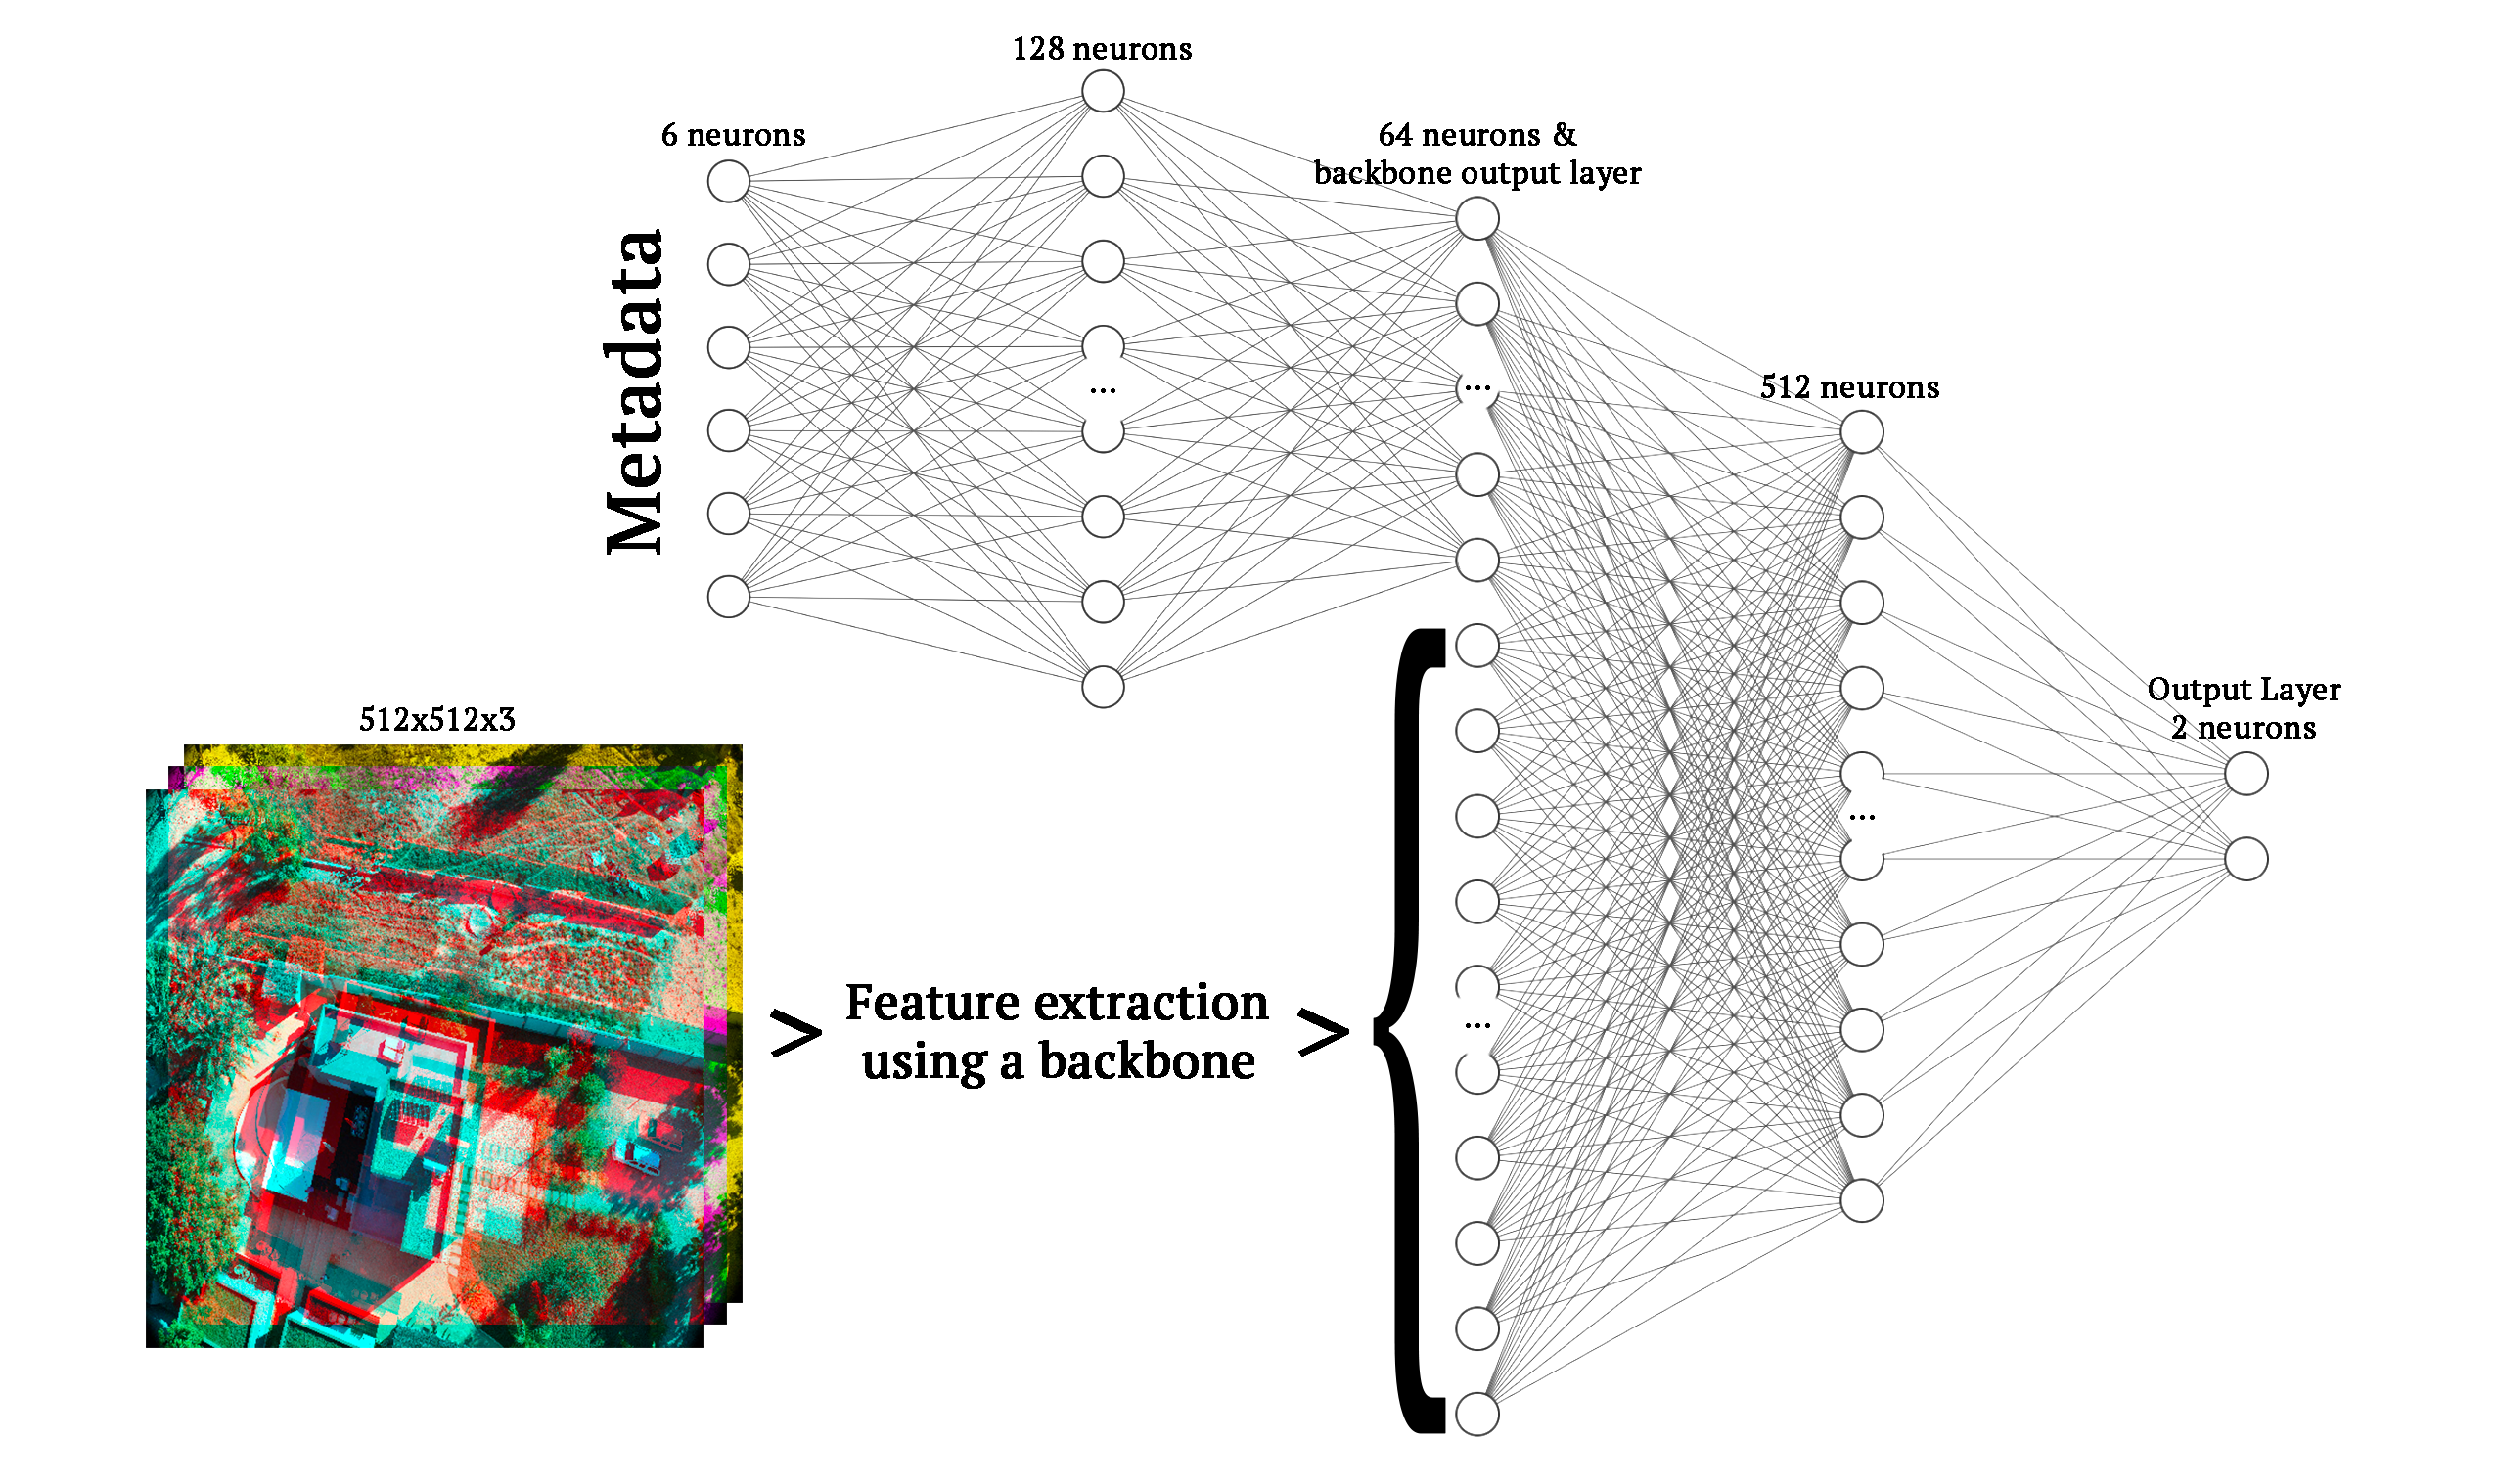
\includegraphics[width=1\linewidth]{assets/nn.png}
    \caption{Architecture of the model shared by user zulo40 in the discussion forums. [ref!]}
    \label{fig:nn}
\end{figure}

After extracting the features they are processed through fully connected layers, where a multi-head attention mechanism is applied after to enhance embeddings. The multi-head attention mechanism is an important technique of CNN from the Transformers architecture, whereby the \textit{attention} (i.e., the importance of certain features) is estimated several times in parallel, allowing to learn different patterns and relationships between different sets of features. Finally a regression head predicts the number of panels (photovoltaic and/or thermal solar) in a given image.
%a arquitetura? desta familia de modelos pode ser verificada na imagem \ref{fig:nn}, que consite num hybrid model de neural networks, ao usar um bacbone (transfer learning) para extrarir features da imagem (cnn's) e snn? para extrar features da metadata. de seguida, é usado um attention head para juntar todas estas features, da imagem e da metadata, para posteriormente obtermos o resultado da regressao

The backbones tested were DenseNet121, EfficientNetv2B3 and ResNet101, and after an initial assessment, EfficientNetv2B3 provided with the best results and the hyperparameters were further fine tuned with the ranges specified in Table \ref{parametroszulp}.

The best set of hyperparameters was selected from a randomized search in a cross validation (CV) set up. Unlike common K-fold CV, due to the long processing times and high computational load, the number of CV repetitions was adjusted 3 times (and not the usual 5 times), and averaged over them. We acknowledge the downside of this approach, particularly the fact that only 66 \% of the data is exposed to validation and the reduced diversity of the models trained. These aspects become particularly evident due to the relatively small size of the dataset.

The criteria for selection of the best model was the MAE (mean absolute error, the metric used in the Zindi challenge), which gave the following hyperparameters marked in bold in Table \ref{parametroszulp}. The hyperparameters were selected for a small number of combinations, given how time consuming training each model is.
%ademais, como backbone foi exprimentado um densenet121, efficientnetv2B3 e resnet101, através da divisao dos dados em treino e validacao e o uso de data augmentation nos dados de treino.

%ao verificar o melhor desempenho pelo efnet, tanto no treino como validacao como teste, decisiu-se fazer um fine-tunning dos hyperparameters.
% JP: A questão do split 80/20 mencionei logo no primeiro parágrafo

\begin{table}[H]
\centering
\caption{Hyperparameter space for the hybrid model \textit{zulo40}. The bold values correspond to the selected hyperparameters.}
\label{parametroszulp}
\begin{tabular}{ll}
\toprule
\textbf{Hyperparameter} & \textbf{Possible Values} \\
\midrule
Batch Size & $\{\mathbf{16}, 32, 64\}$ \\
Optimizer & \textbf{AdamW} \\
Learning Rate & $[\mathbf{10^{-5}}, 10^{-3}]$ \\
Weight Decay & $[\mathbf{10^{-5}}, 10^{-3}]$ \\
Dropout & $\{0.2, 0.3, \mathbf{0.4}\}$ \\
Scheduler & \textbf{CosineAnnealingWarmRestarts} \\
T\_0 & $\{3, \mathbf{5}, 7, 10\}$ \\
T\_mult & $\{1, \mathbf{2}, 3, 5\}$ \\
Loss & \textbf{HuberLoss} \\
$\delta$ & \textbf{1} \\
\bottomrule
\end{tabular}
\end{table}


%na tabela \ref{parametroszulp} pode se verificar o espaco possivel de hyperparametros utilizado, tendo sido a escolha dos melhores baseada numa random search com o uso de cross-validation.

%contudo esta cross validation não foi muito tipica devido aos elevados tempos de ajuste dos modelos. os dados de treino foram separados em 5 folds (80/20), mas cada conjunto de hyperparametros so foi ajustado 3 vezes, e não as tipicas 5 vezes.


%de modo a escolher o melhor modelo usou-se o validation mae médio como métrica tendo sido o melhor conjunto de hyperparametros dado por 
\begin{comment}
- batch 16

- leraning 1e-4

- weight dec 1e-4

- dropout 0.4

- t0 5

- tmul 2

meta06
\end{comment}

%para alem disso é tbm importante indicar o uso de: 

%- juntar os modelos (3, pq sao 3 folds) e faz a media das previsoes

Upon selecting the best model, the final inference on the test data was done resorting to TTA, Test-Time Augmentation, where the model makes multiple predictions on augmented versions of the same image (e.g., flipping, scaling, cropping). With this, the final result is an average of the group of predictions. The scheduler selected (CosineAnnealingWarmRestarts) dynamically changes the learning rate following a cosine schedule, with a defined period (T\_0 = 5), where at each period the learning rate decays to a minimum, restarting at the highest set learning rate. This allows to prevent locking into local minima, by passing through higher learning rates periodically, allowing for fine tuning with lower learning rates for longer periods (given T\_mult = 2, where the period increases two fold at each restart).

The erratic behaviour of the CV loss curve is evident from Fig. \ref{fig:model01_lc}, likely due to the small validation set (20 \% of an already small dataset), which leads to variance spikes due to the changing samples within. The training loss is rather smooth, with periodical increases well in line with the scheduler's algorithm (5, 5 + 10, 15 + 20, ...).
%- Test-Time Augmentation (TTA), where the model makes multiple predictions on augmented versions of the same image (e.g., flipping, scaling, cropping). These predictions are later averaged to improve accuracy.

%- o scheduler altera o learning rate e o paraetro de regularizacao

%quanto aos resultados deste modelo ...

\begin{figure}[H]
    \centering
    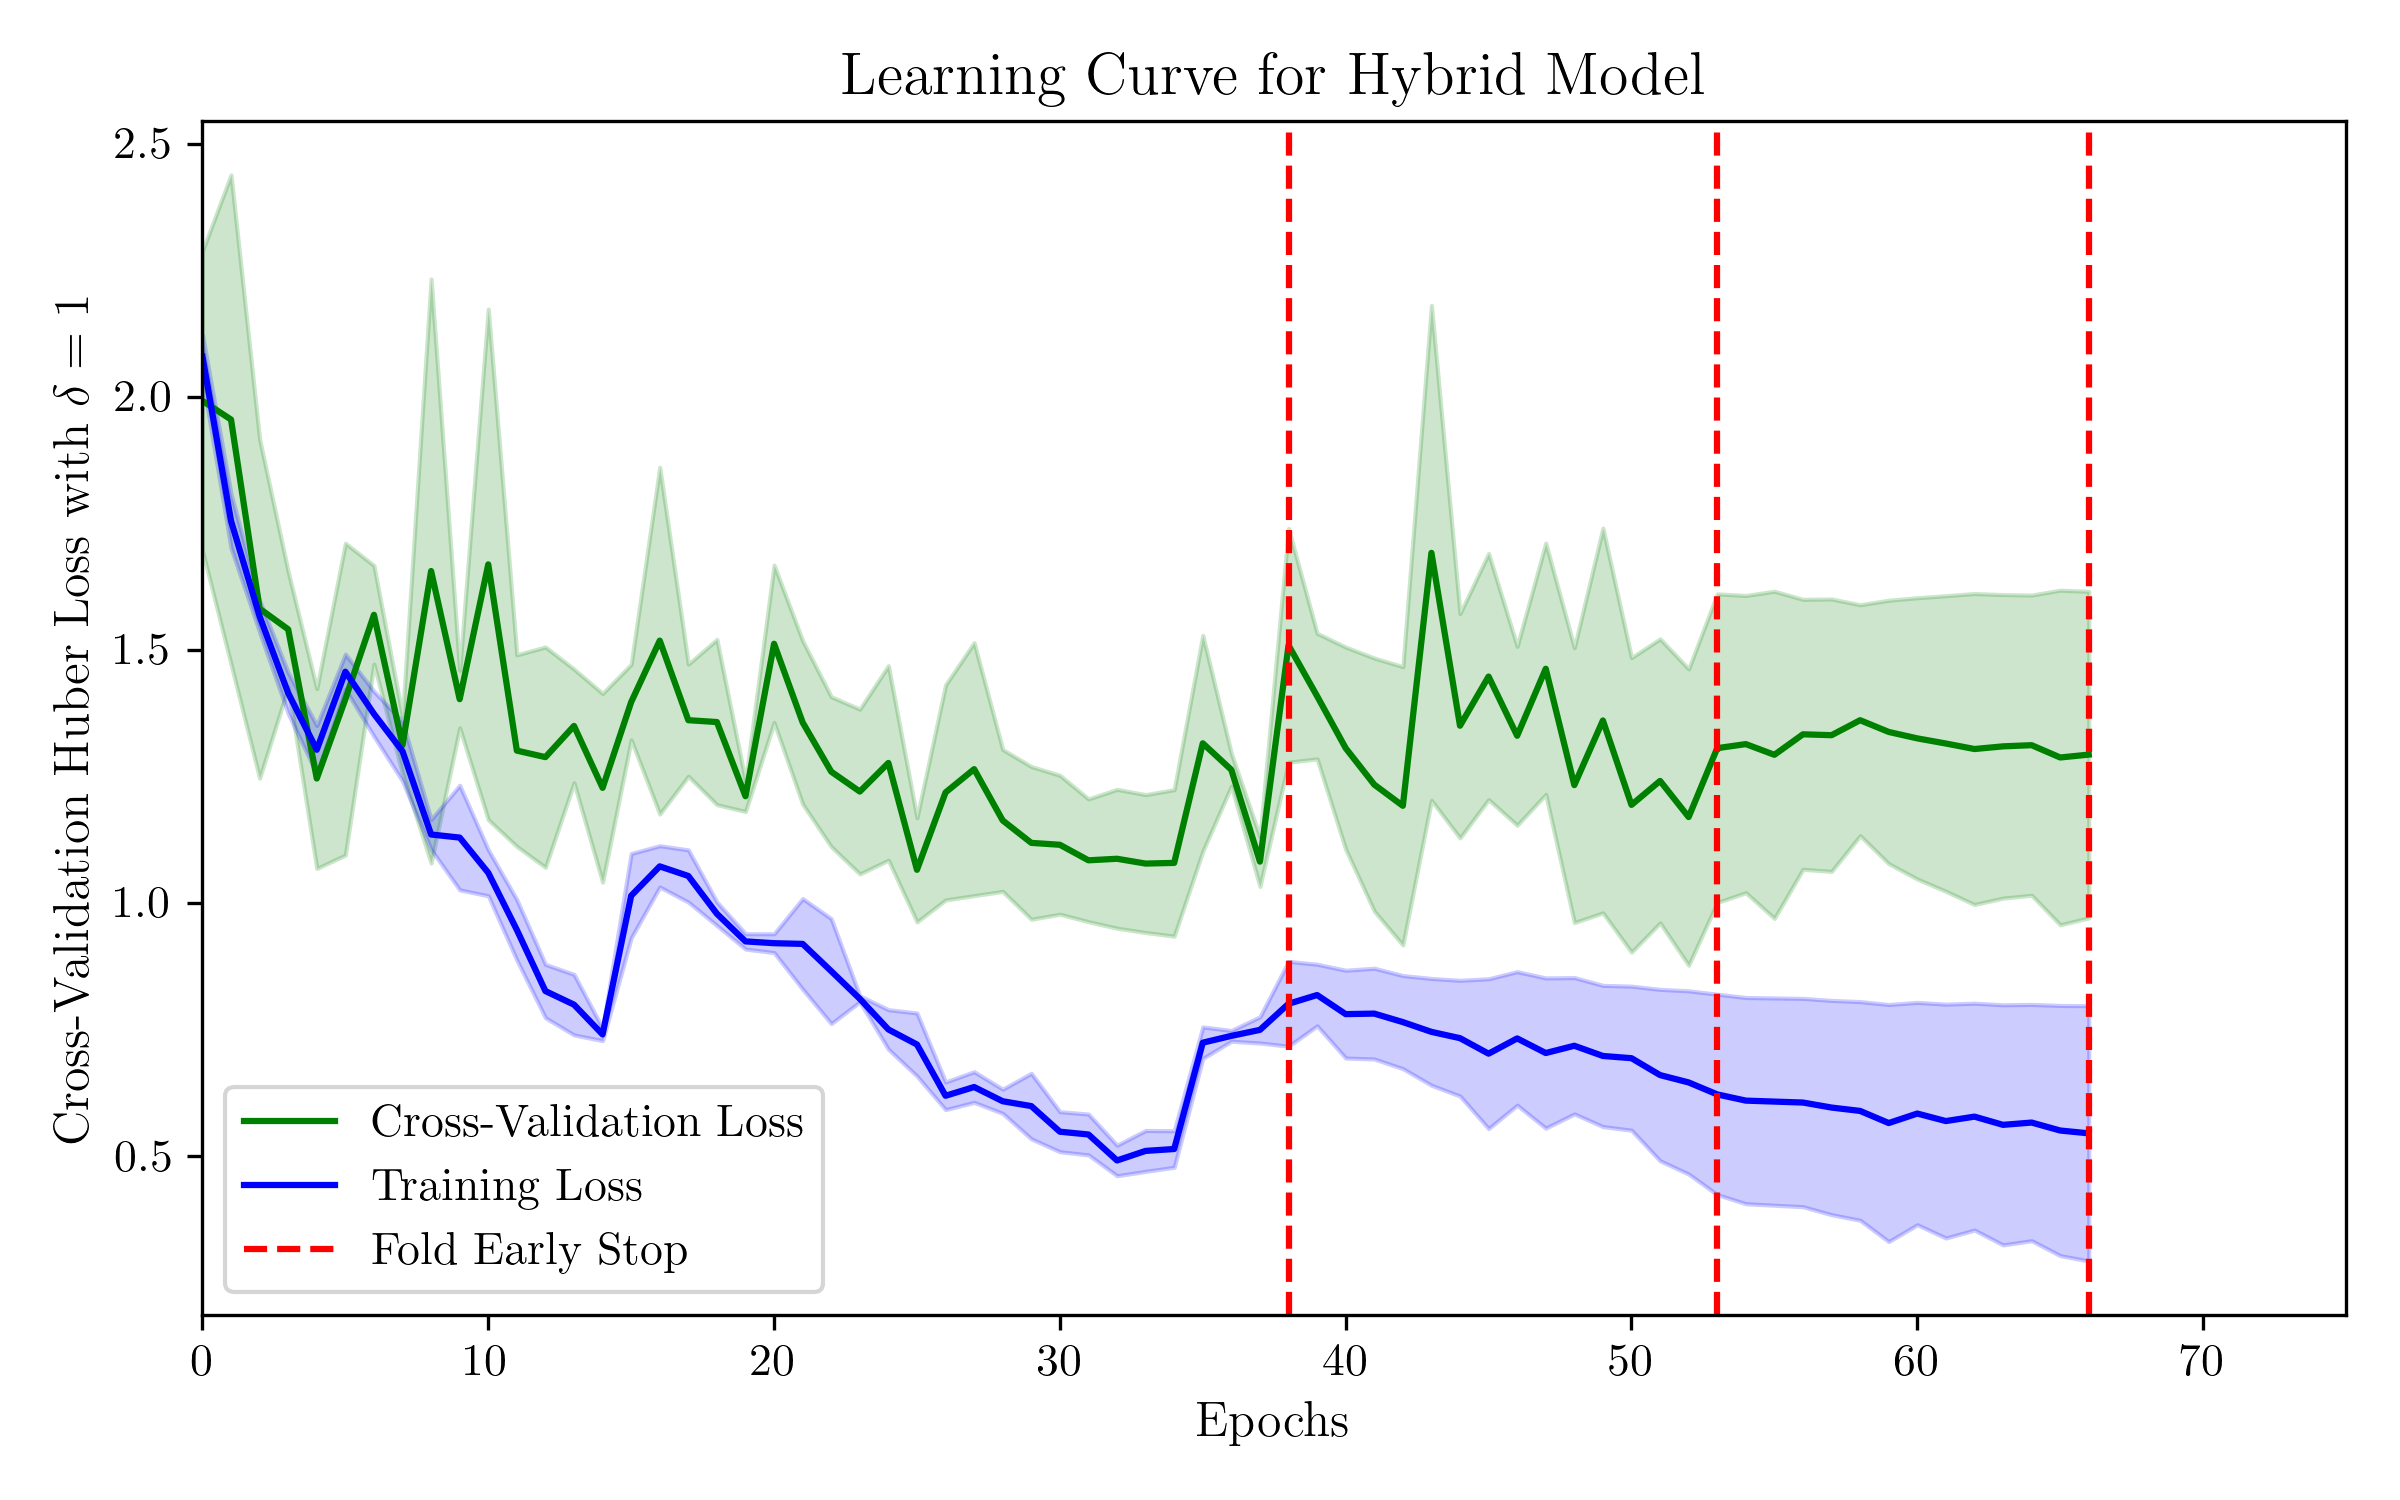
\includegraphics[width=1\linewidth]{assets/model01_lc.png}
    \caption{Learning curve for the \textit{zulo40} hydrid model, with Training and Cross-Validation Loss plotted (with standard deviation in shade).}
    \label{fig:model01_lc}
\end{figure}

%a learning curve Fig. \ref{fig:model01_lc}.... é de notar q ela revela picos em certar epochs (porximo da 5, 15, 35) devido ao scheduler aumentar o parametro de regularizacao 
%JP: o scheduler não mexe com o parâmetro de regularização

The training proceeded for 75 epochs, where the best model was selected based on the best validation MAE. From the learning curve, it does not seem to be overfit, but considering the MAE metric and the test set from the Zindi challenge, the test MAE is considerably higher than the training MAE (Table \ref{tab:model01_results}, indicating that the model is not capable of generalizing so well.

%para alem disso a mesma parou a epoch 66 por early stopping, sendo o criterio de paragem a melhor validation mae (ns se e early stopping pq n tem patience mas sim max de 75 epochs e dps escolher o melhor)

%no signs of overffiting

\begin{table}[H]
\centering
\caption{Error metrics for the Hybrid Model, for the train and test set, along with the number of samples for each.}
\label{tab:model01_results}
\begin{tabular}{lccc}
\toprule
\textbf{Dataset} & \textbf{MAE} & \textbf{Support} \\
\midrule
Train Set & 0.5127 & 3312 \\
Test Set & 0.8434 & 1107 \\
\bottomrule
\end{tabular}
\end{table}

%quanto as metricas de erro presentes na Table \ref{tab:model01_results}, apesar de so termos o MAE parece n haver sinais de overiffing pelas medidas serem semelhantes
% JP: considerando que o erro no dataset de teste é um bom bocado pior, parece-me estar overfit, já que o modelo não consegue generalizar muito bem
% HV: estamos a falar de falhar 0.3 paineis por imagem, continua a arredondar para o 0, diria q signnigicativo só a partir de valores proximos de 1 ou superiores. a metrica q tens uma indica q em media dizes +- .5 paineis e a outra +- .8, não é algo percentual, é absoluto, dai nao achar significativo
\subsection{Object Detection}

\textbf{isto tbm é do yolo de obj seg, ns onde se meta:} ideia inicial era fazer segmentacao de conjuntos de paineis e de boilers e posteriormente com outro modelo fazer contagem. problema foi q o modelo ao reconhecer paineis invidivudais, mesmo em conjuntos identificava individuais, levando ao mau desempenho do modelo

entao decidiu-se rever o dataset e separar manualmente os poligonos em paineis e boileres indivudais, deixando de existir grupos de paineis

o yolo apresentou assim mt melhores resultados, apesar da reducao da dimensao do dataset em termos de imagens mas aumento de amostras do que realmente sao paineis e boilers individuais

\textbf{le o instance segmentation, o inicio, antes de começares este, so para ver se ha algo q se deva puxar para aqui}

bla bla, pesquisa de hyperperamentros

yolos dedicados a bonding boxes, object detetcion.....


\begin{table}[H]
\centering
\caption{yolo obj id model hyp}
\label{parametrosobjid}
\begin{tabular}{ll}
\toprule
\textbf{Hyperparameter} & \textbf{Possible Values} \\
\midrule
Batch Size conta? & $\{16, 32\}$ \\
yolo & \{yolo11l, yolo11m, yolov8l\} \\
imgsize & 512 \\
augment & True \\
patiente & $[15, 25]$ \\
cls & $[0.5, 1.5]$ \\
lr0 & $[10^{-5}, 10^{-3}]$ \\
lrf & $[0.1, 1]$ \\
mixup & $[0, 0.75]$ \\
copy\_paste & $[0, 0.75]$ \\
scale & $[0.5, 1]$ \\
\bottomrule
\end{tabular}
\end{table}

after fitting multiple models with the same type of cv said above

\begin{figure}[H]
    \centering
    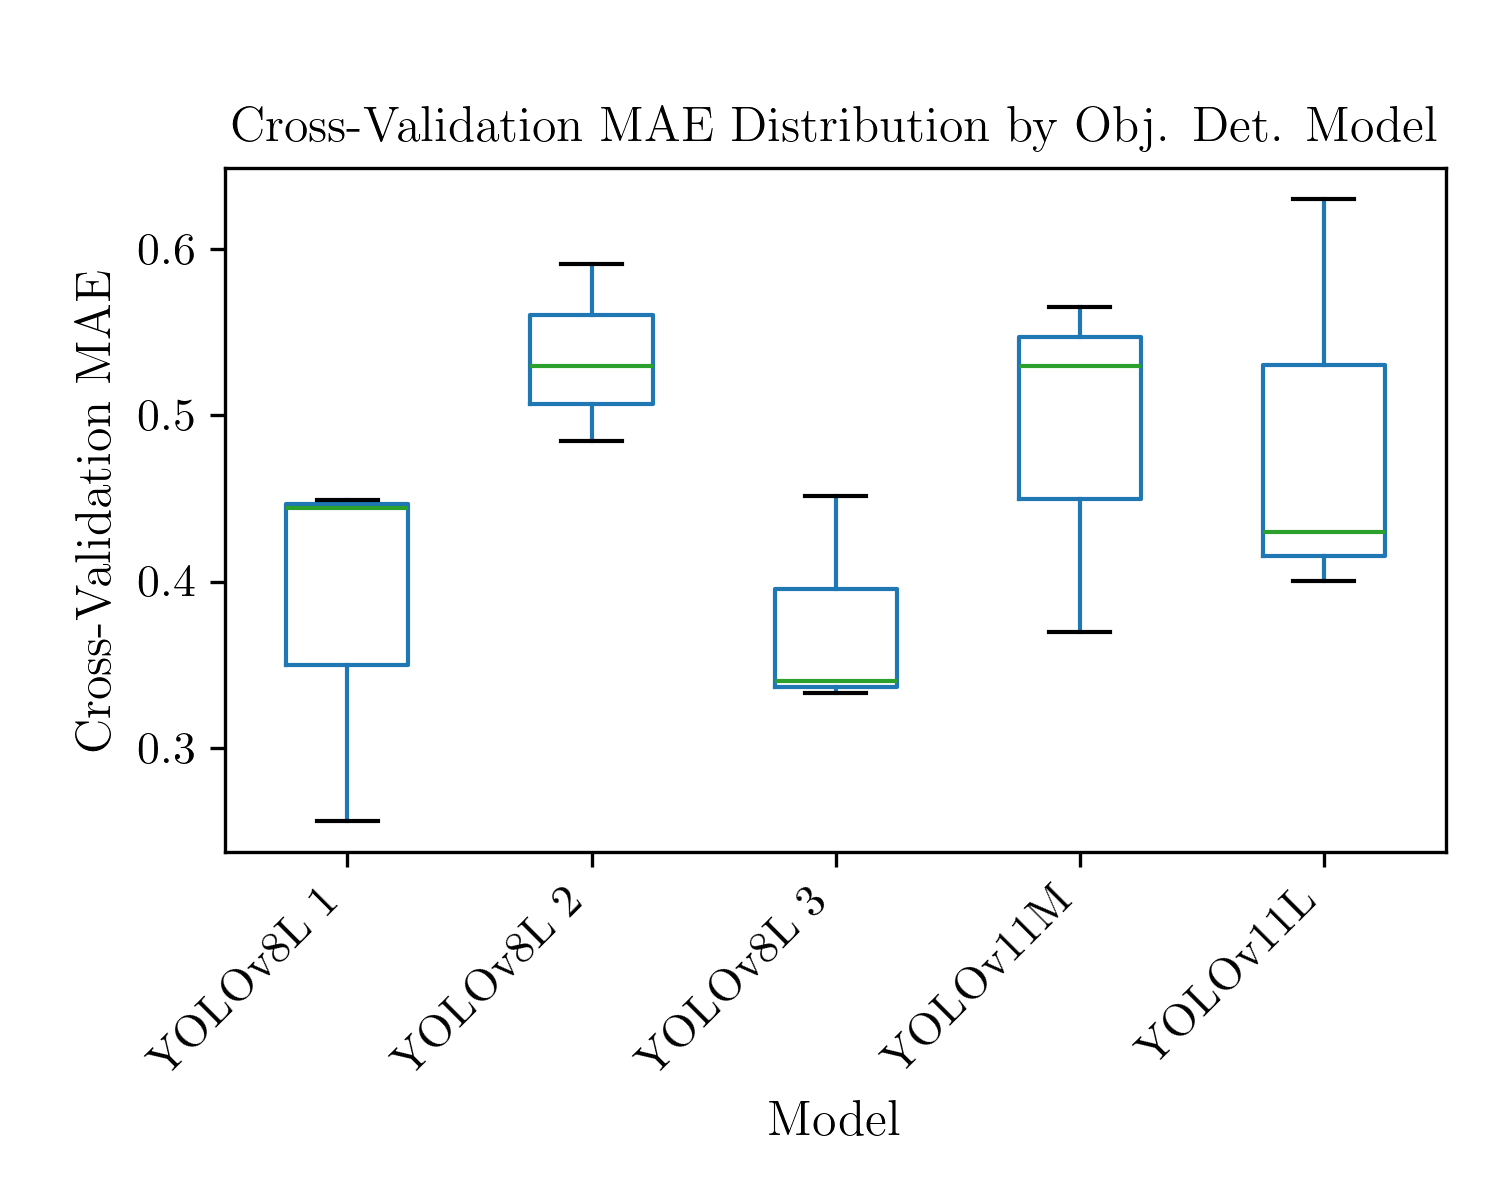
\includegraphics[width=1\linewidth]{assets/model03_mae_boxplot.png}
    \caption{CAPTION CAPTION CAPTION CAPTION CAPTION}
    \label{fig:model03_mae_boxplot}
\end{figure}

% MODEL03 = OBJ ID pq foi a ordem que fizemos na realidade (nao a do report)

with yolov8l 3 with the lowest mean mae, the best hyperparemteres were

- yolov8L
- batch 32
- imgsize 512
- agument True
- patient 20
- cls 1.5
- lr0 2e-4
- lrf 1
- mixup 0.75
- copypaste 0.75
- scale 0.9

and the other hyperparameteres fixed to the deafult of ultralytics yolov8L model


\textbf{copia do yolo seg:}
quanto aos resultados do modelo em referencia, é de notar que o mesmo foi treinado tendo em conta o segmentar os objetos (pan e boilers) da melhor forma possivel, pelo que as metricas do ajuste do modelo sao referentes a isso e nao ao problema de contagem, sendo esta contagem apenas feita apos o modelo ajustar os segmentos as imagens

\begin{figure}[H]
    \centering
    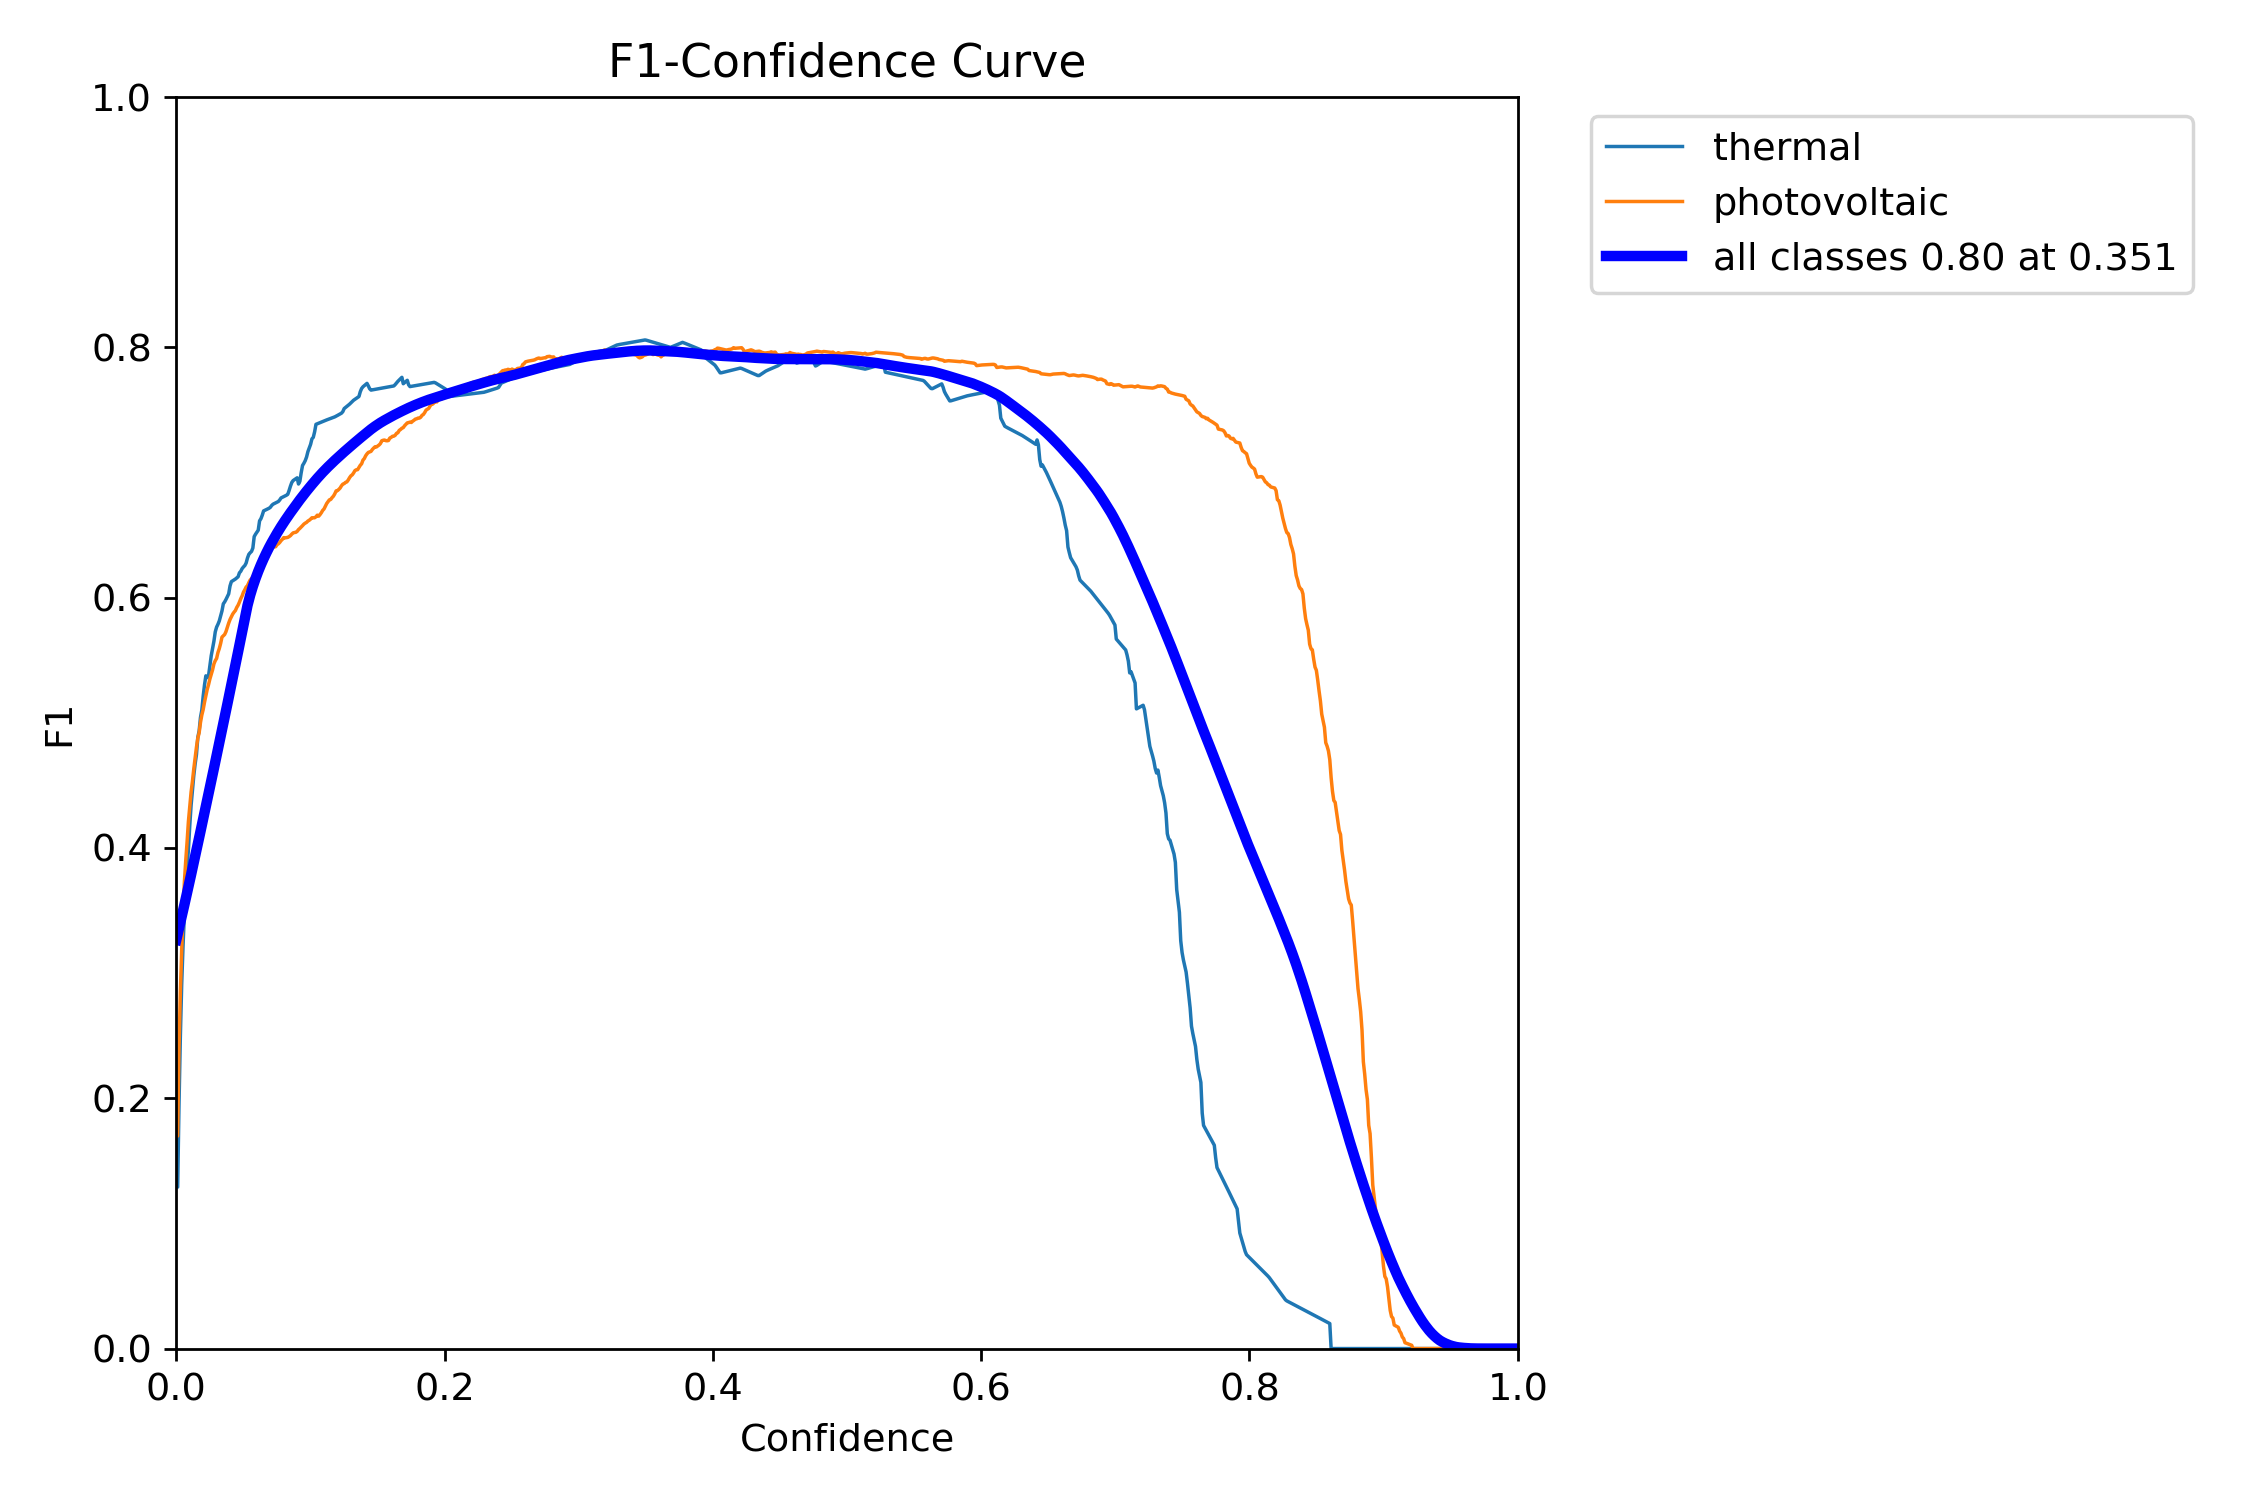
\includegraphics[width=1\linewidth]{assets/model03_yolof1.png}
    \caption{CAPTION CAPTION CAPTION CAPTION CAPTION (gerado pelo modulo do yolo automaticamente) referir isso pq ele é "diferente" dos outros ig}
    \label{fig:model03_yolof1}
\end{figure}

bla bla tudo bem, bem proximos....

learning curve

\begin{figure}[H]
    \centering
    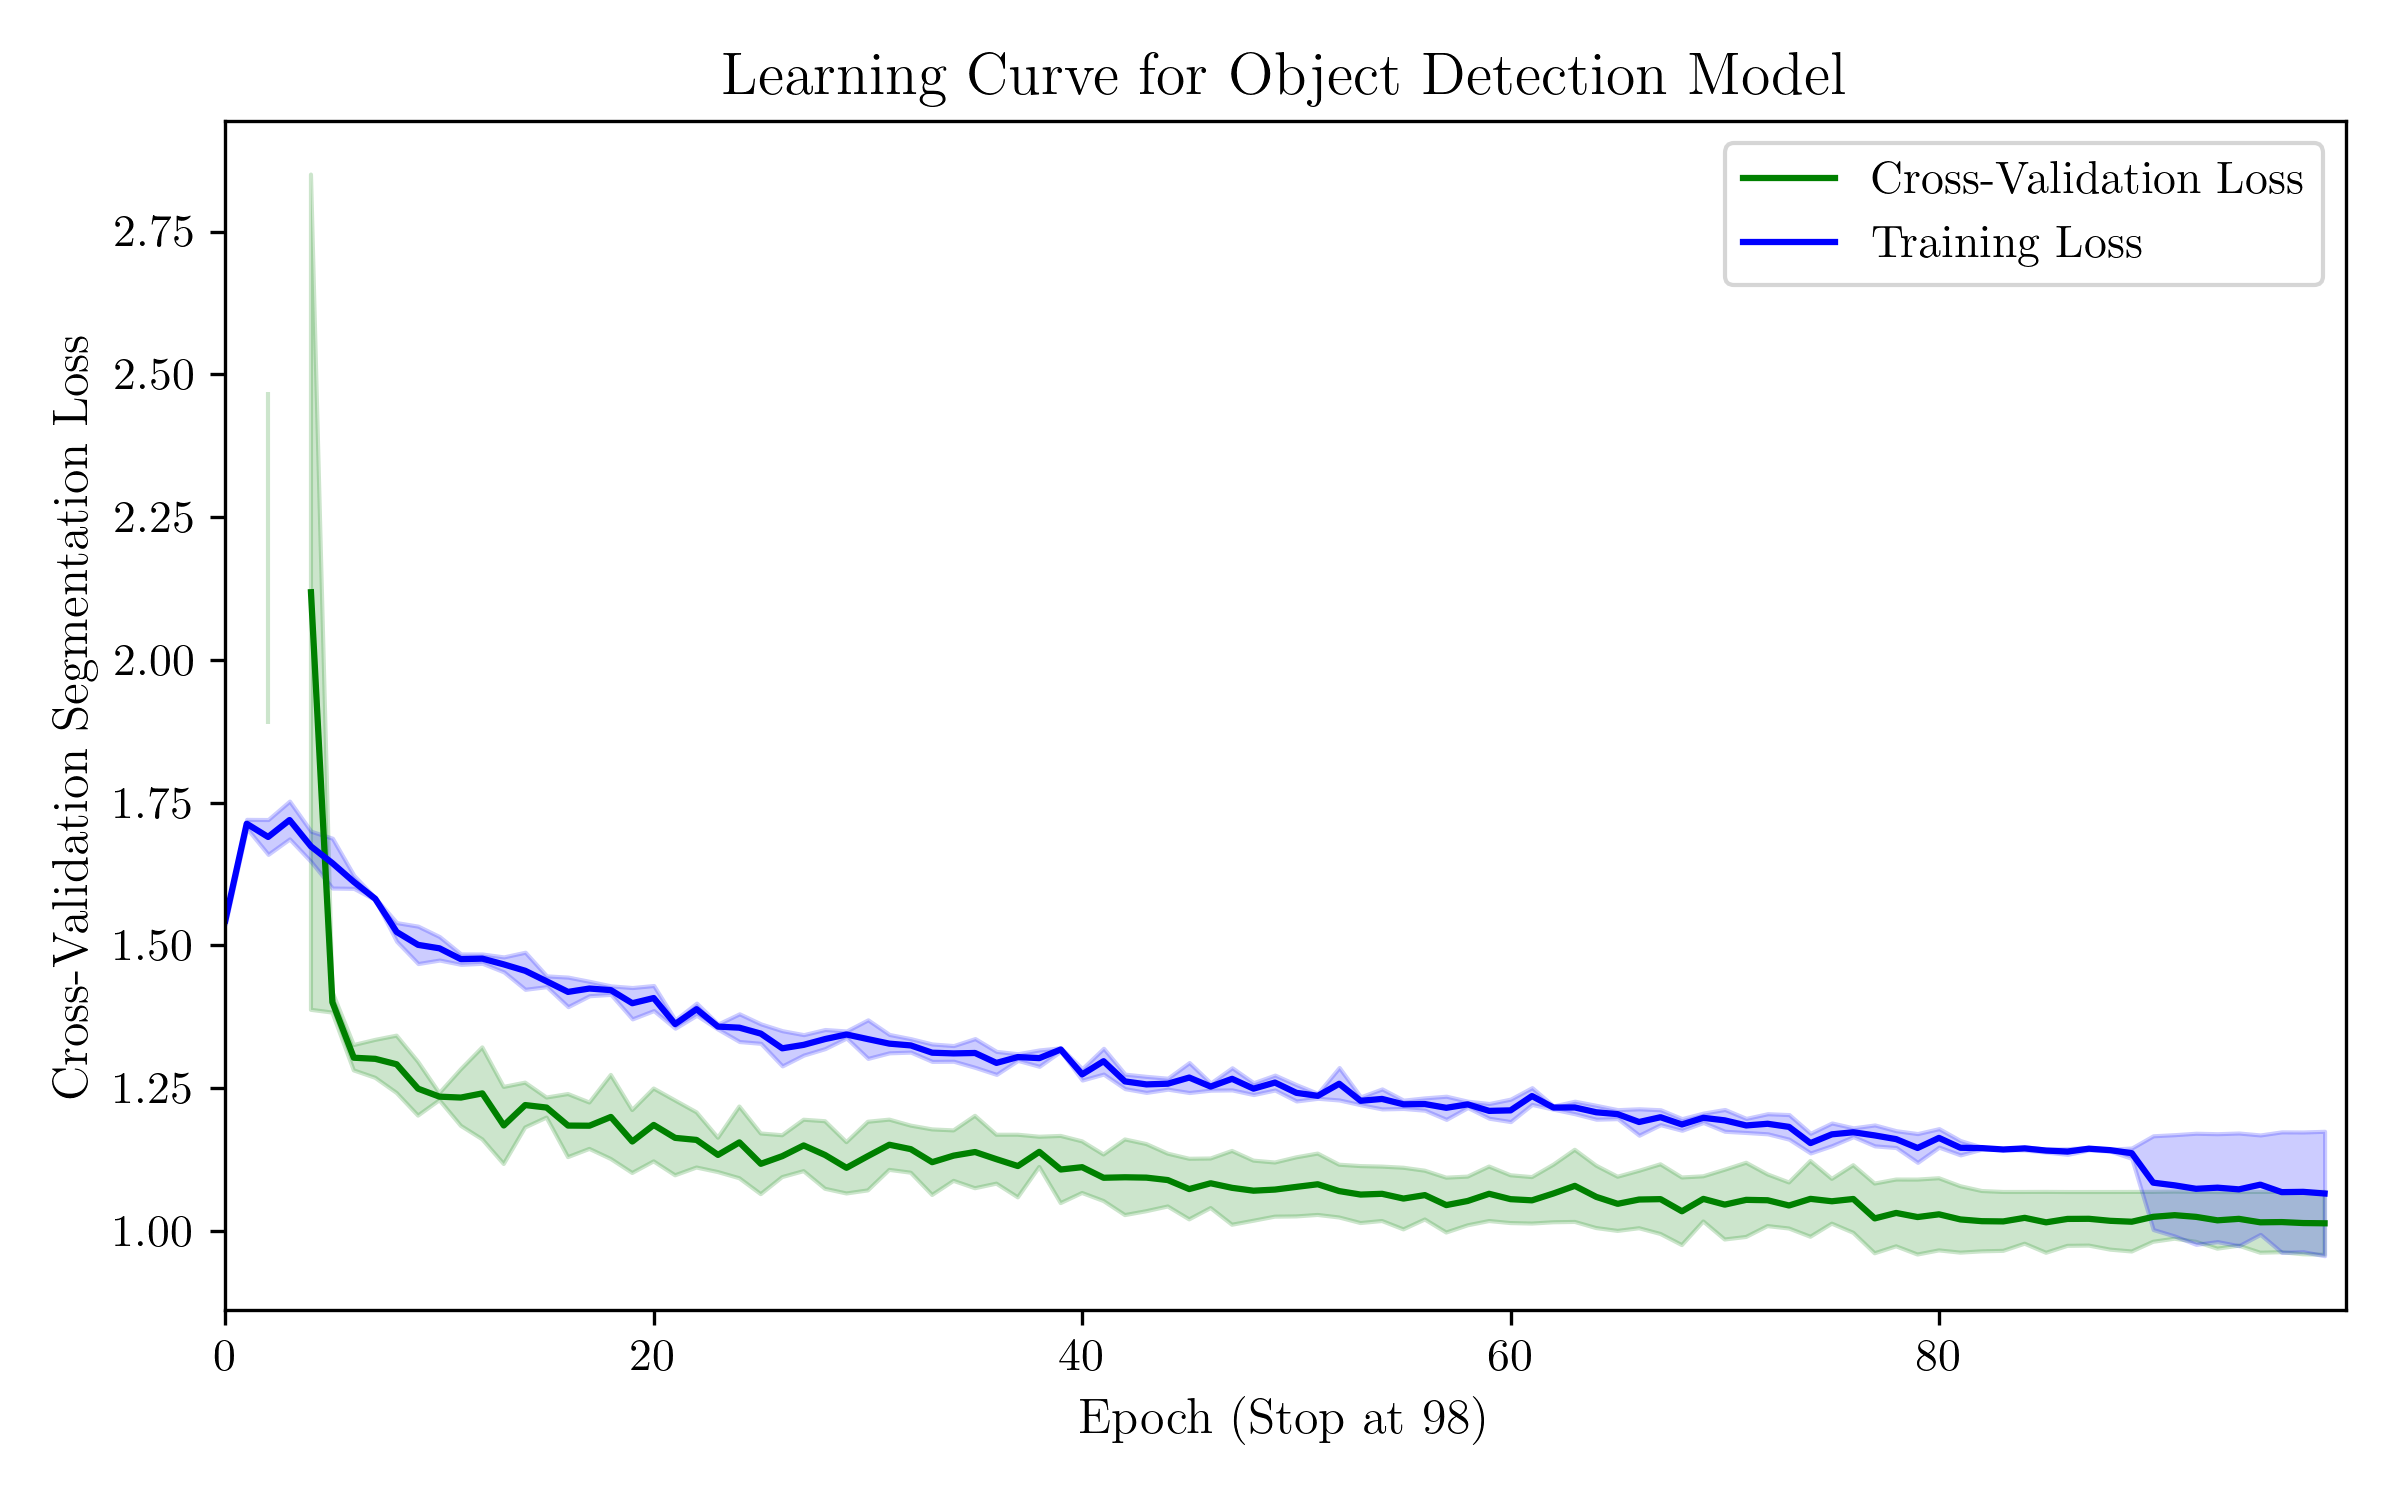
\includegraphics[width=1\linewidth]{assets/model03_lc.png}
    \caption{CAPTION CAPTION CAPTION CAPTION CAPTION}
    \label{fig:model03_lc}
\end{figure}

sem sinais de overfitting

\begin{table}[H]
\centering
\caption{Error metrics for the Object Detection Model, for the train and test set, along with the number of samples for each.}
\label{tab:model02_results}
\begin{tabular}{lccc}
\toprule
\textbf{Dataset} & \textbf{MAE} & \textbf{Support} \\
\midrule
Train Set & XXXXXX & 3312 \\
Test Set & XXXXXX & 1107 \\
\bottomrule
\end{tabular}
\end{table}







\subsection{Instance Segmentation}


de modo a encontrar o melhor modelo de segmentacao dos paineis e boilers, tal como no efnet (depende se vem dps ou antes) os dados foram dividicos em 5 folds, e para cada conjunto de hyperparametros os modelos foram ajustados em 3 conjuntos diferentes de 4 folds sendo validado no restante, e o modelo escolhido foi aaquele com menor mae médio nos folds de validacao

o conjunto de pesquisa de hyperparemetros é dado pela tabela seguinte, mas é de notar q nsao sao testadas todas as combinacoes mas apenas algumas aleatorias


\begin{table}[H]
\centering
\caption{yolo seg model hyp}
\label{parametrosseg}
\begin{tabular}{ll}
\toprule
\textbf{Hyperparameter} & \textbf{Possible Values} \\
\midrule
Batch Size conta? & $\{8, 32, 16\}$ \\
yolo & \{yolo11l-seg, yolo11m-seg, yolov8l-seg\} \\
imgsize & 512 \\
augment & True \\
patiente & $[10, 25]$ \\
cls & $[0.5, 2.5]$ \\
lr0 & $[10^{-4}, 10^{-3}]$ \\
lrf & $[0.01, 0.1, 1]$ \\
mixup & $[0, 0.5]$ \\
copy\_paste & $[0, 0.8]$ \\
scale & $[0.5, 1]$ \\
\bottomrule
\end{tabular}
\end{table}

\begin{figure}[H]
    \centering
    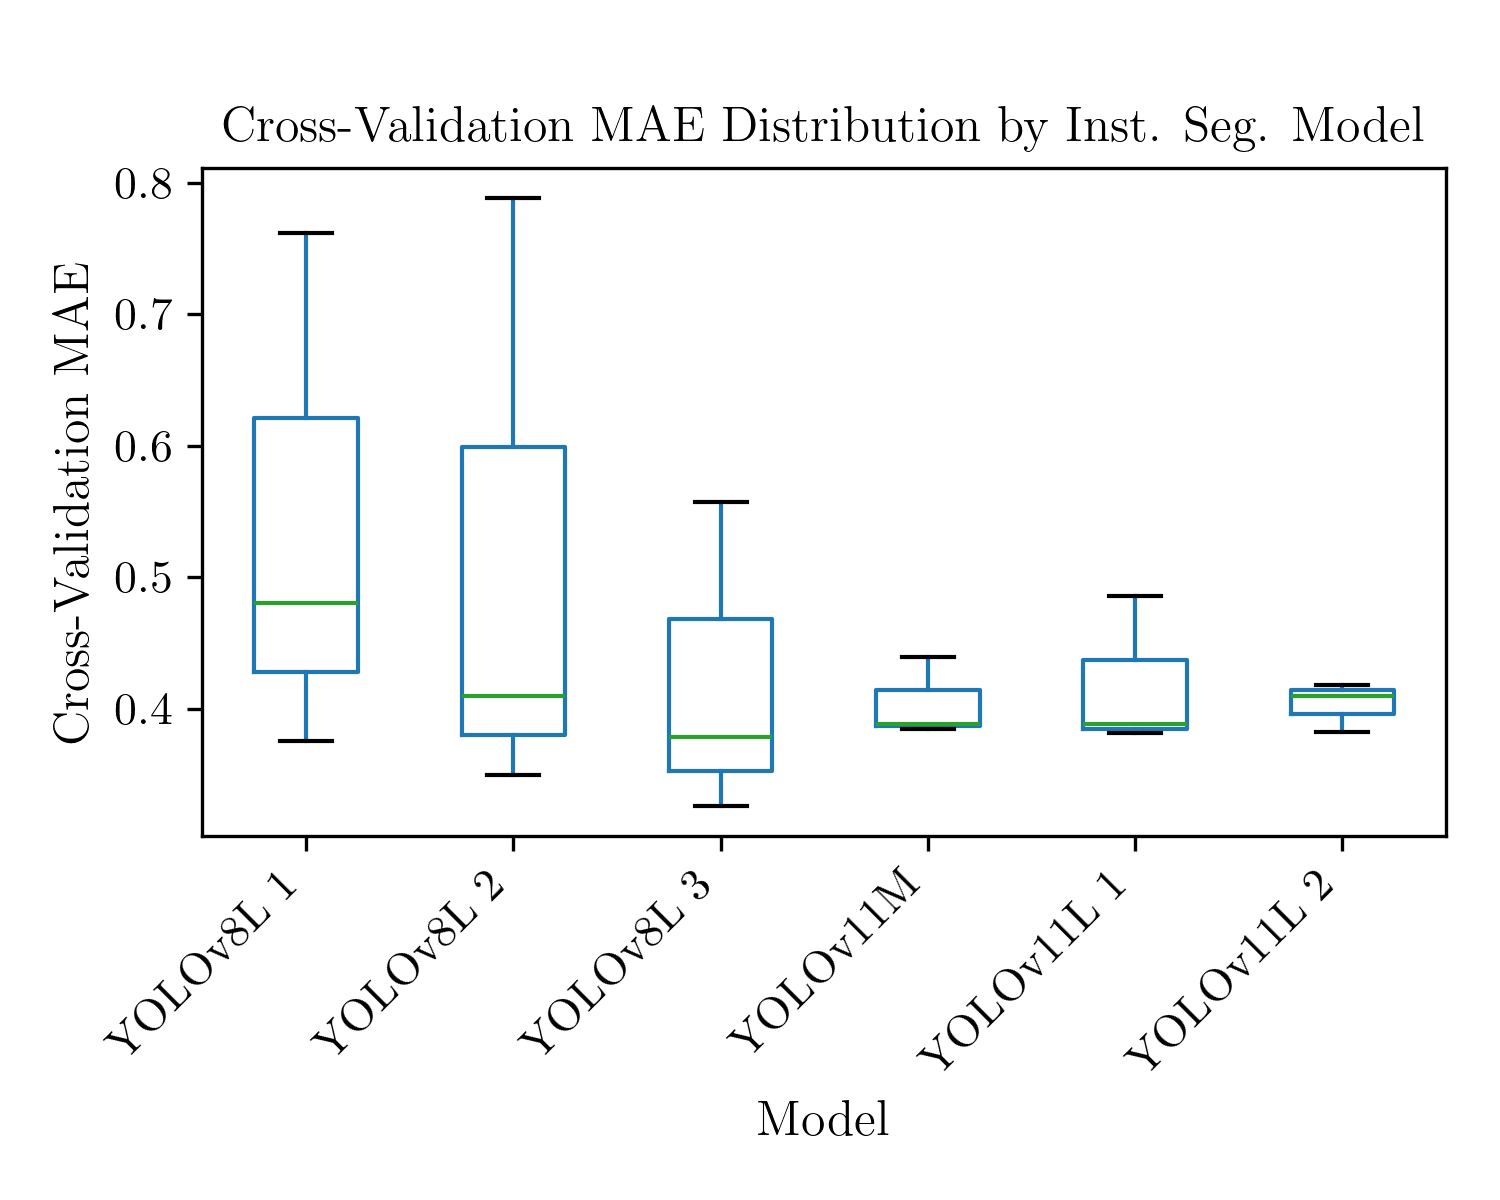
\includegraphics[width=1\linewidth]{assets/model02_mae_boxplot.png}
    \caption{CAPTION CAPTION CAPTION CAPTION CAPTION}
    \label{fig:model02_mae_boxplot}
\end{figure}

a fig \ref{fig:model02_mae_boxplot} demonstra o mae para os diferentes modelos ajustados na busca dos melhores hyperparemtros, tendo sido o YOLOv11L 2 a obter o menos MAE médio nas suas validações, tendo sido ele o escolhido. seguem-se abaixo os seus hyperparemetros

- yolo yolo11l-seg
- imgsize 512
- augment True
- patiente 25
- lr0 $10^{-3}$
- lrf 0.1
- cls 0.5
- mixup 0
- copy paste 0
- scale 0.5

os restantes parametros sao os que vêm por defeito no package ultralytics
%https://github.com/ultralytics/ultralytics
referentes ao modelo yolo11l-seg

quanto aos resultados do modelo em referencia, é de notar que o mesmo foi treinado tendo em conta o segmentar os objetos (pan e boilers) da melhor forma possivel, pelo que as metricas do ajuste do modelo sao referentes a isso e nao ao problema de contagem, sendo esta contagem apenas feita apos o modelo ajustar os segmentos as imagens

\begin{figure}[H]
    \centering
    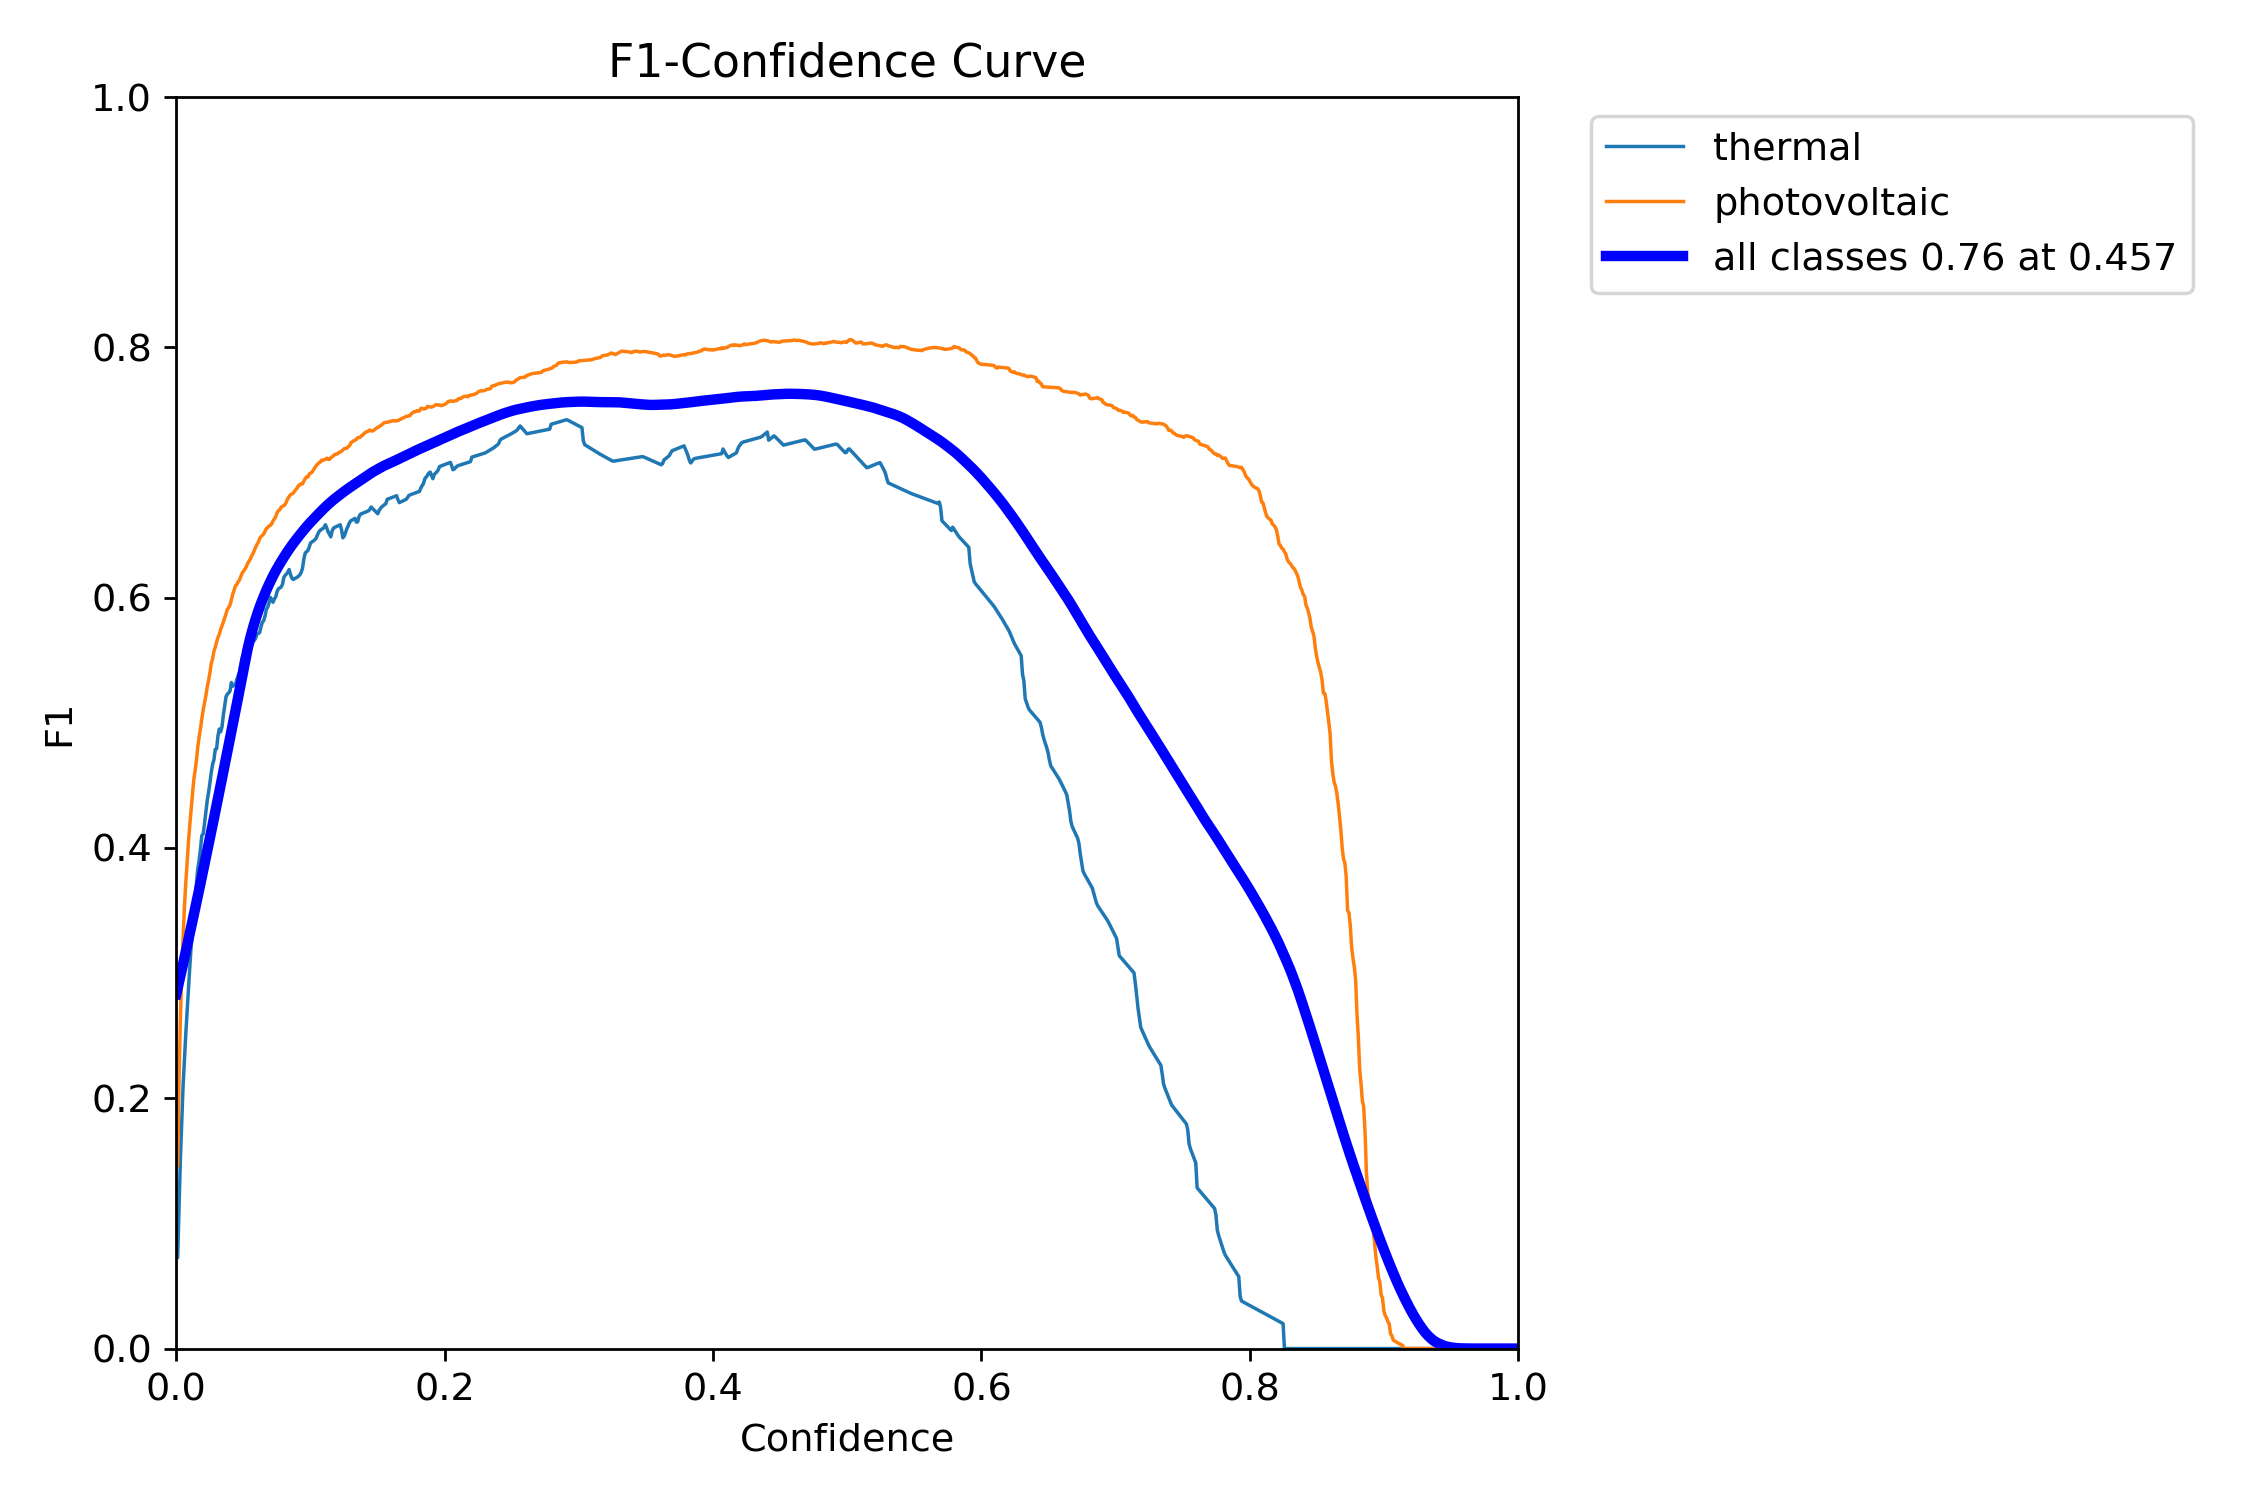
\includegraphics[width=1\linewidth]{assets/model02_yolof1.png}
    \caption{CAPTION CAPTION CAPTION CAPTION CAPTION (gerado pelo modulo do yolo automaticamente) referir isso pq ele é "diferente" dos outros ig}
    \label{fig:model02_yolof1}
\end{figure}

a fig. \ref{fig:model02_yolof1} mostra a metrica f1 relativa a segemntacao do segundo fold do modelo, revelando um melhor desempenho dos photovoltaic em relacao aos thermal, mas sem uma diferenca significativa.

\begin{figure}[H]
    \centering
    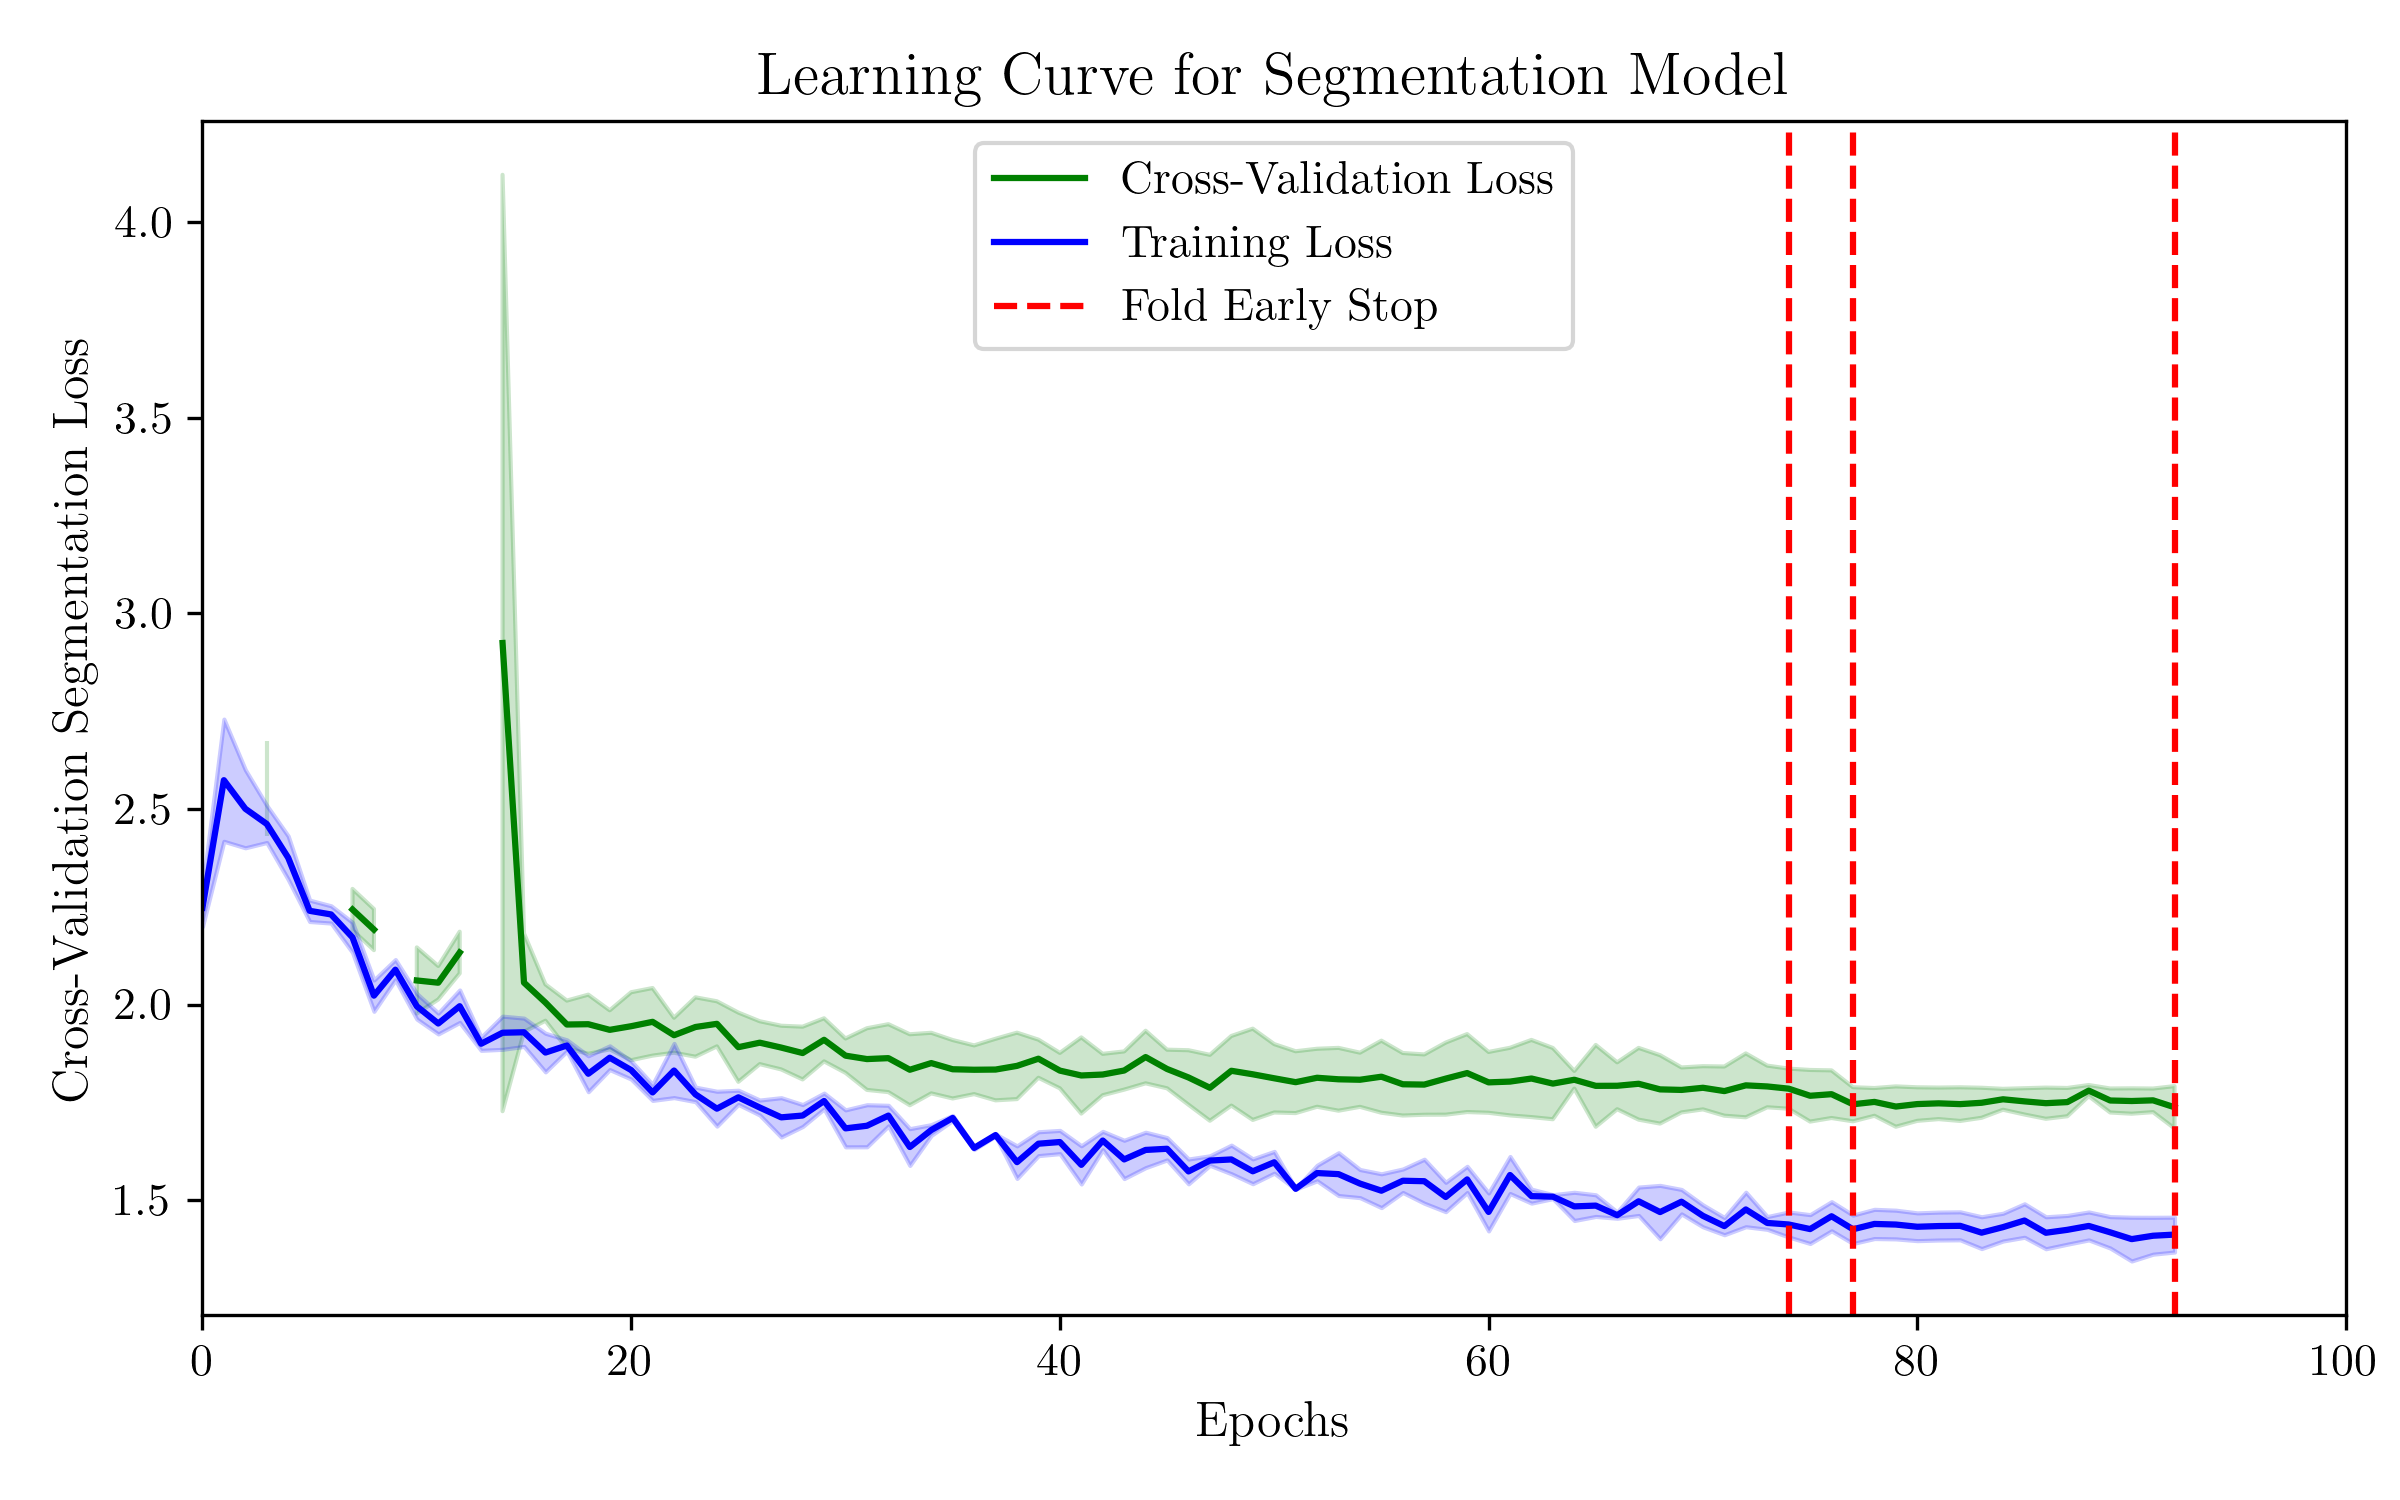
\includegraphics[width=1\linewidth]{assets/model02_lc.png}
    \caption{CAPTION CAPTION CAPTION CAPTION CAPTION}
    \label{fig:model02_lc}
\end{figure}

na fig. \ref{fig:model02_lc} pode-se verificar a learning curve do melhor modelo, a demonstrar a sua convergencia sem sinais de overiffint. apenas com um possivel outlier na loss, que pode ter devido a algum erro de computacao por parte do calculo do segmentation loss por parte do yolo. é possível ver tbm a paragem do modelo após 92 epochs por early stopping.

\begin{table}[H]
\centering
\caption{Error metrics for the Segmentation Model, for the train and test set, along with the number of samples for each.}
\label{tab:model02_results}
\begin{tabular}{lccc}
\toprule
\textbf{Dataset} & \textbf{MAE} & \textbf{Support} \\
\midrule
Train Set & 1.5645 & 3312 \\
Test Set & 1.3415 & 1107 \\
\bottomrule
\end{tabular}
\end{table}

quanto as metricas relacionadas com a contagem dos pan e boil, o nosso problema original, o seu resultado é apresentado na tabela \ref{tab:model02_results}


\section{Discussion} 

https://zindi.africa/competitions/lacuna-solar-survey-challenge/discussions/25674

\subsection{Performance Metrics}

discussao


\section{Conclusion}

conc


\section*{Work Load}

Both authors contributed equally to the project.

\bibliographystyle{IEEEtran}
\bibliography{references}

\end{document}



